
\documentclass[12pt]{report}
\usepackage[utf8]{inputenc}
\usepackage{graphicx}
\usepackage{listings}
\usepackage{lstautogobble}
\graphicspath{ {images/} }
\usepackage{float}
\floatstyle{boxed} 
\restylefloat{figure}

\begin{document}

\title{
	{Tendermint: Byzantine Fault Tolerance in the Age of Blockchains}\\
	{\large University of Guelph}\\
}

\author{Ethan Buchman}
\date{\today}

\maketitle

\clearpage
\thispagestyle{plain}
\par\vspace*{.35\textheight}{\centering Dedicated to Theda. \par}

\chapter*{Abstract}
Tendermint is a new protocol for ordering events in a distributed network under adversarial conditions.
More commonly known as consensus or atomic broadcast, the problem has attracted significant attention
recently due to the widespread success of digital currencies, such as Bitcoin and Ethereum,
which successfully solve the problem in public settings without a central authority.
Tendermint modernizes classic academic work on the subject to provide a secure consensus protocol with 
accountability guarantees, as well as an interface for building arbitrary applications above the consensus.
Tendermint is high performance, achieving thousands of transactions per second on dozens of nodes distributed around the globe,
with latencies of about one second, and performance degrading moderately in the face of adversarial attacks.

\chapter*{Preface}
The structure and presentation of this thesis was directly inspired by Diego Ongaro's 2014 Doctoral Dissertation, 
``Consensus: Bridging Theory and Practice'', wherein he specifies and evaluates the Raft consensus algorithm.

Much of the work done in this thesis was done in collaboration with Jae Kwon, who initiated the Tendermint project.
Please see the Github repository, at https://github.com/tendermint/tendermint, for a more direct account of contributions to the codebase.


\chapter*{Acknowledgements}
I learned early in life from Tony Montana that a man has only two things in this world, his word and his balls, and he should break em for nobody.
This thesis would not have been completed if I had not given my word to certain people that I would complete it.
These include my family, in particular my parents, grandparents, and great uncle Paul, and my primary advisor, Graham,
who has, for one reason or another, permitted me a practically abusive amount of flexibility to pursue the topic of my choosing.
Thanks Graham.

Were it not for another set of individuals, this thesis would probably have been about machine learning.
These include Vlad Zamfir, with whom I have experienced countless moments of discovery and insight;
My previous employer and favorite company, Eris Industries, and especially their CEO and COO, Casey Kuhlman and Preston Byrne,
for hiring me, mentoring me, and giving me such freedom to research and tinker and ultimately start my own company with technology they helped fund;
Jae Kwon, for his direct mentorship in consensus science and programming, for being a great collaborator, and for being the core founder and CEO at Tendermint;
Zach Ramsay, for being, for all intents and purposes, my heterosexual husband;
and of course, Satoshi Nakamoto, whomever you are, for sending me down this damned rabbit hole in the first place.

There are of course many other people who have influenced my life during the course of this graduate degree;
you know who you are, and I thank you for being that person and for all you've done for me.

\pagenumbering{roman}
\tableofcontents
\listoffigures
\listoftables
\pagenumbering{arabic}

\chapter{Introduction}
\label{ch:intro}

The cold, hard truth about computer engineering today is that computers are faulty - 
they crash, corrupt, slow down, perform voodoo. 
What's worse, we're typically interested in connecting computers over a network (like the internet),
and networks can be more unpredictable than the computers themselves.
These challenges are primarily the concern of "fault tolerant distributed computing",
whose aim is to discover principled protocol designs enabling faulty computers communicating over a faulty network 
to stay in sync while providing a useful service.
In essence, to make a reliable system from unreliable parts.

In an increasingly digital and globalized world, however, 
systems must not only be reliable in the face of unreliable parts, but in the face of malicious or "Byzantine" ones.
Over the last decade, major components of critical infrastructure have been ported to networked systems,
as have vast components of the world's finances.
In response, there has been an explosion of cyber warfare and financial fraud,
and a complete distortion of economic and political fundamentals.

In 2009, an anonymous sofware developer known only as Satoshi Nakamoto introduced an approach to the resolution of these issues 
that was simultaneously an experiment in computer science, economics, and politics. 
It was a digital currency called Bitcoin \cite{bitcoin}.
Bitcoin was the first protocol to solve the problem of fault tolerant distributed computing in the face of malicious adversaries in a public setting.
The solution, dubbed a "blockchain", hosts a digital currency, 
where consent on the order of transactions is negotiated via an economically incentivized cryptographic random lottery based on partial hash collisions.
In essence, transactions are ordered in batches (blocks) by those who find partial hash collisions of the transaction data, 
in such a way that the correct ordering is the one where the collisions have the greatest cumulative difficulty.
The solution was dubbed Proof-of-Work (PoW).

Bitcoin's subtle brilliance was to invent a currency, a cryptocurrency, and to issue it to those solving the hash collisions, 
in exchange for their doing such an expensive thing as solve partial hash collisions \cite{cost_of_mining}.
In spirit, it might be assumed that the capacity to solve such problems would be distributed as computing power is, 
such that anyone with a CPU could participate.
Unfortunately, the reality is that the Bitcoin network has grown into the largest supercomputing entity on the planet, greater than all others combined,
evaluating only a single function, distributed across a few large data centers running Application Specific integrated circuits (ASICs) produced by a small number of primarily Chinese companies, and consuming on the order of X kW per transaction.
Not to mention it takes up to an hour to confirm transactions, is difficult to build on top of, and does not scale in a way which preserves its security guarantees.
This is not to mention the internal bout of political struggles resulting from the immaturity of the Bitcoin community's governance mechaninisms.

Despite these troubles, Bitcoin, astonishingly, continues to churn,
and its technology, 
of cryptography and distributed databases and co-operative economics,
continues to attract billions in investment capital,
both in the form of new companies and new cryptocurrencies,
each diverging from Bitcoin in its own unique way.

In 2014, Jae Kwon began the development of Tendermint, which sought to solve the consensus problem,
of ordering and executing a set of transactions in an adversarial environment, 
by modernizing solutions to the problem that have existed for decades,
but have lacked the social context to be deployed widely until now.

In early 2015, in an effort led by Eris Industries to bring a practical blockchain solution to industry,
the author joined Jae Kwon in the development of the Tendermint software and protocols.

The result of that collaboration is the Tendermint platform, consisting of a consensus protocol, a high-performance implementation in golang, 
a flexible interface for building arbitrary applications above the consensus, and a suite of tools for deployments and their management.
We believe Tendermint achieves a superior design and implementation compared to previous approaches, 
including that of the classical academic literature \cite{dls,pbft,raft} as well as Bitcoin \cite{bitcoin} and its derivatives \cite{ethereum,sidechains,peercoin}
by combining the right elements of each to achieve a practical balance of security, performance, and simplicity.
We have since started a company to pursue the deployment of the platform at an enterprise level, and have seen tremendous interest.

The primary contributions of this thesis are as follows:


\begin{itemize}  

    \item A complete description of the Tendermint consensus algorithm and platform architecture (Chapters \ref{ch:tendermint}-\ref{ch:apps}). Tendermint provides provably optimal Byzantine Fault Tolerant consensus, is easy to understand and reason about, flexible to build on top of, and provides a foundation for advanced and secure socio-political and economic systems. 

    \item Significant contributions to a high performance implementation of the consensus algorithm in Golang, most notably a refactor of the core consensus state machine to be more robust, deterministic, and understandable, as well as countless bug fixes and performance improvements.

    \item Evaluation of the implementation's performance and characteristics in normal, faulty, and malicious conditions on large deployments (Chapter \ref{ch:performance}). Tendermint consensus is mostly asynchronous, with minimal dependence on synchronized clocks, and can tolerate up to a third of its nodes behaving arbitrarily. 

    \item Discussion and contributions to implementation of many other elements necessary for a complete system, such as membership changes, crisis recovery, client design, and security (Chapters \ref{ch:client} and \ref{ch:governance}).

    \item An informal proof of correctness and directions for more formal approaches (Chapter \ref{ch:tendermint}).

    \item An explanation of blockchains and the Tendermint consensus algorithm in the context of classical academic consensus research (Chapter \ref{ch:related}).
\end{itemize}

All code is available open source at https://github.com/tendermint/tendermint, and in associated repositories at https://github.com/tendermint. 
The core is licensed GPLv3 and most of the libraries are Apache 2.0.

The remainder of this thesis introduces the consensus problem, 
classic solutions, and motivates Tendermint (Chapter \ref{ch:motivation});
presents the Tendermint consensus algorithm, 
the peer-to-peer network, 
and the interface for building arbitrary applications on top 
(Chapters \ref{ch:tendermint}-\ref{ch:apps});
mechanisms for governance and membership changes, and how clients interact with Tendermint (Chapters \ref{ch:governance} and \ref{ch:clients});
outlines the implementation in Golang and evaluates its fault tolerance and performance (Chapters \ref{ch:implementation} and \ref{ch:performance});
and discusses related work (Chapter \ref{ch:related}).

\chapter{Motivation}
\label{ch:motivation}

Distributed consensus systems have become a critical component of modern internet infrastructure, powering every major internet application at some level or another.

The most common paradigm for studying and implementing distributed consensus is that of the Replicated State Machine, 
wherein a \emph{deterministic} state machine is replicated across a set of nodes, 
such that it functions as a single state machine despite the failure of some nodes.
The state machine is driven by a set of inputs, known as \emph{transactions}, 
where each transaction may or may not, depending on its validity, cause a state transition and return a result.
The state transition logic is governed by the state machine's state transition function,
which maps a transaction and the current state to a new state and a return value.
The state transition function is also sometimes referred to as \emph{application logic}.

It is the responsibility of the consensus protocol to order the transactions so that the resulting 
\emph{transaction log} is replicated exactly on every node.
Using a deterministic state transition function implies that 
every node will compute the same state given the same transaction log.

A summary of the replicated state machine architecture is given in Figure \ref{fig:replicated_state_machine}.

\begin{figure}[]
	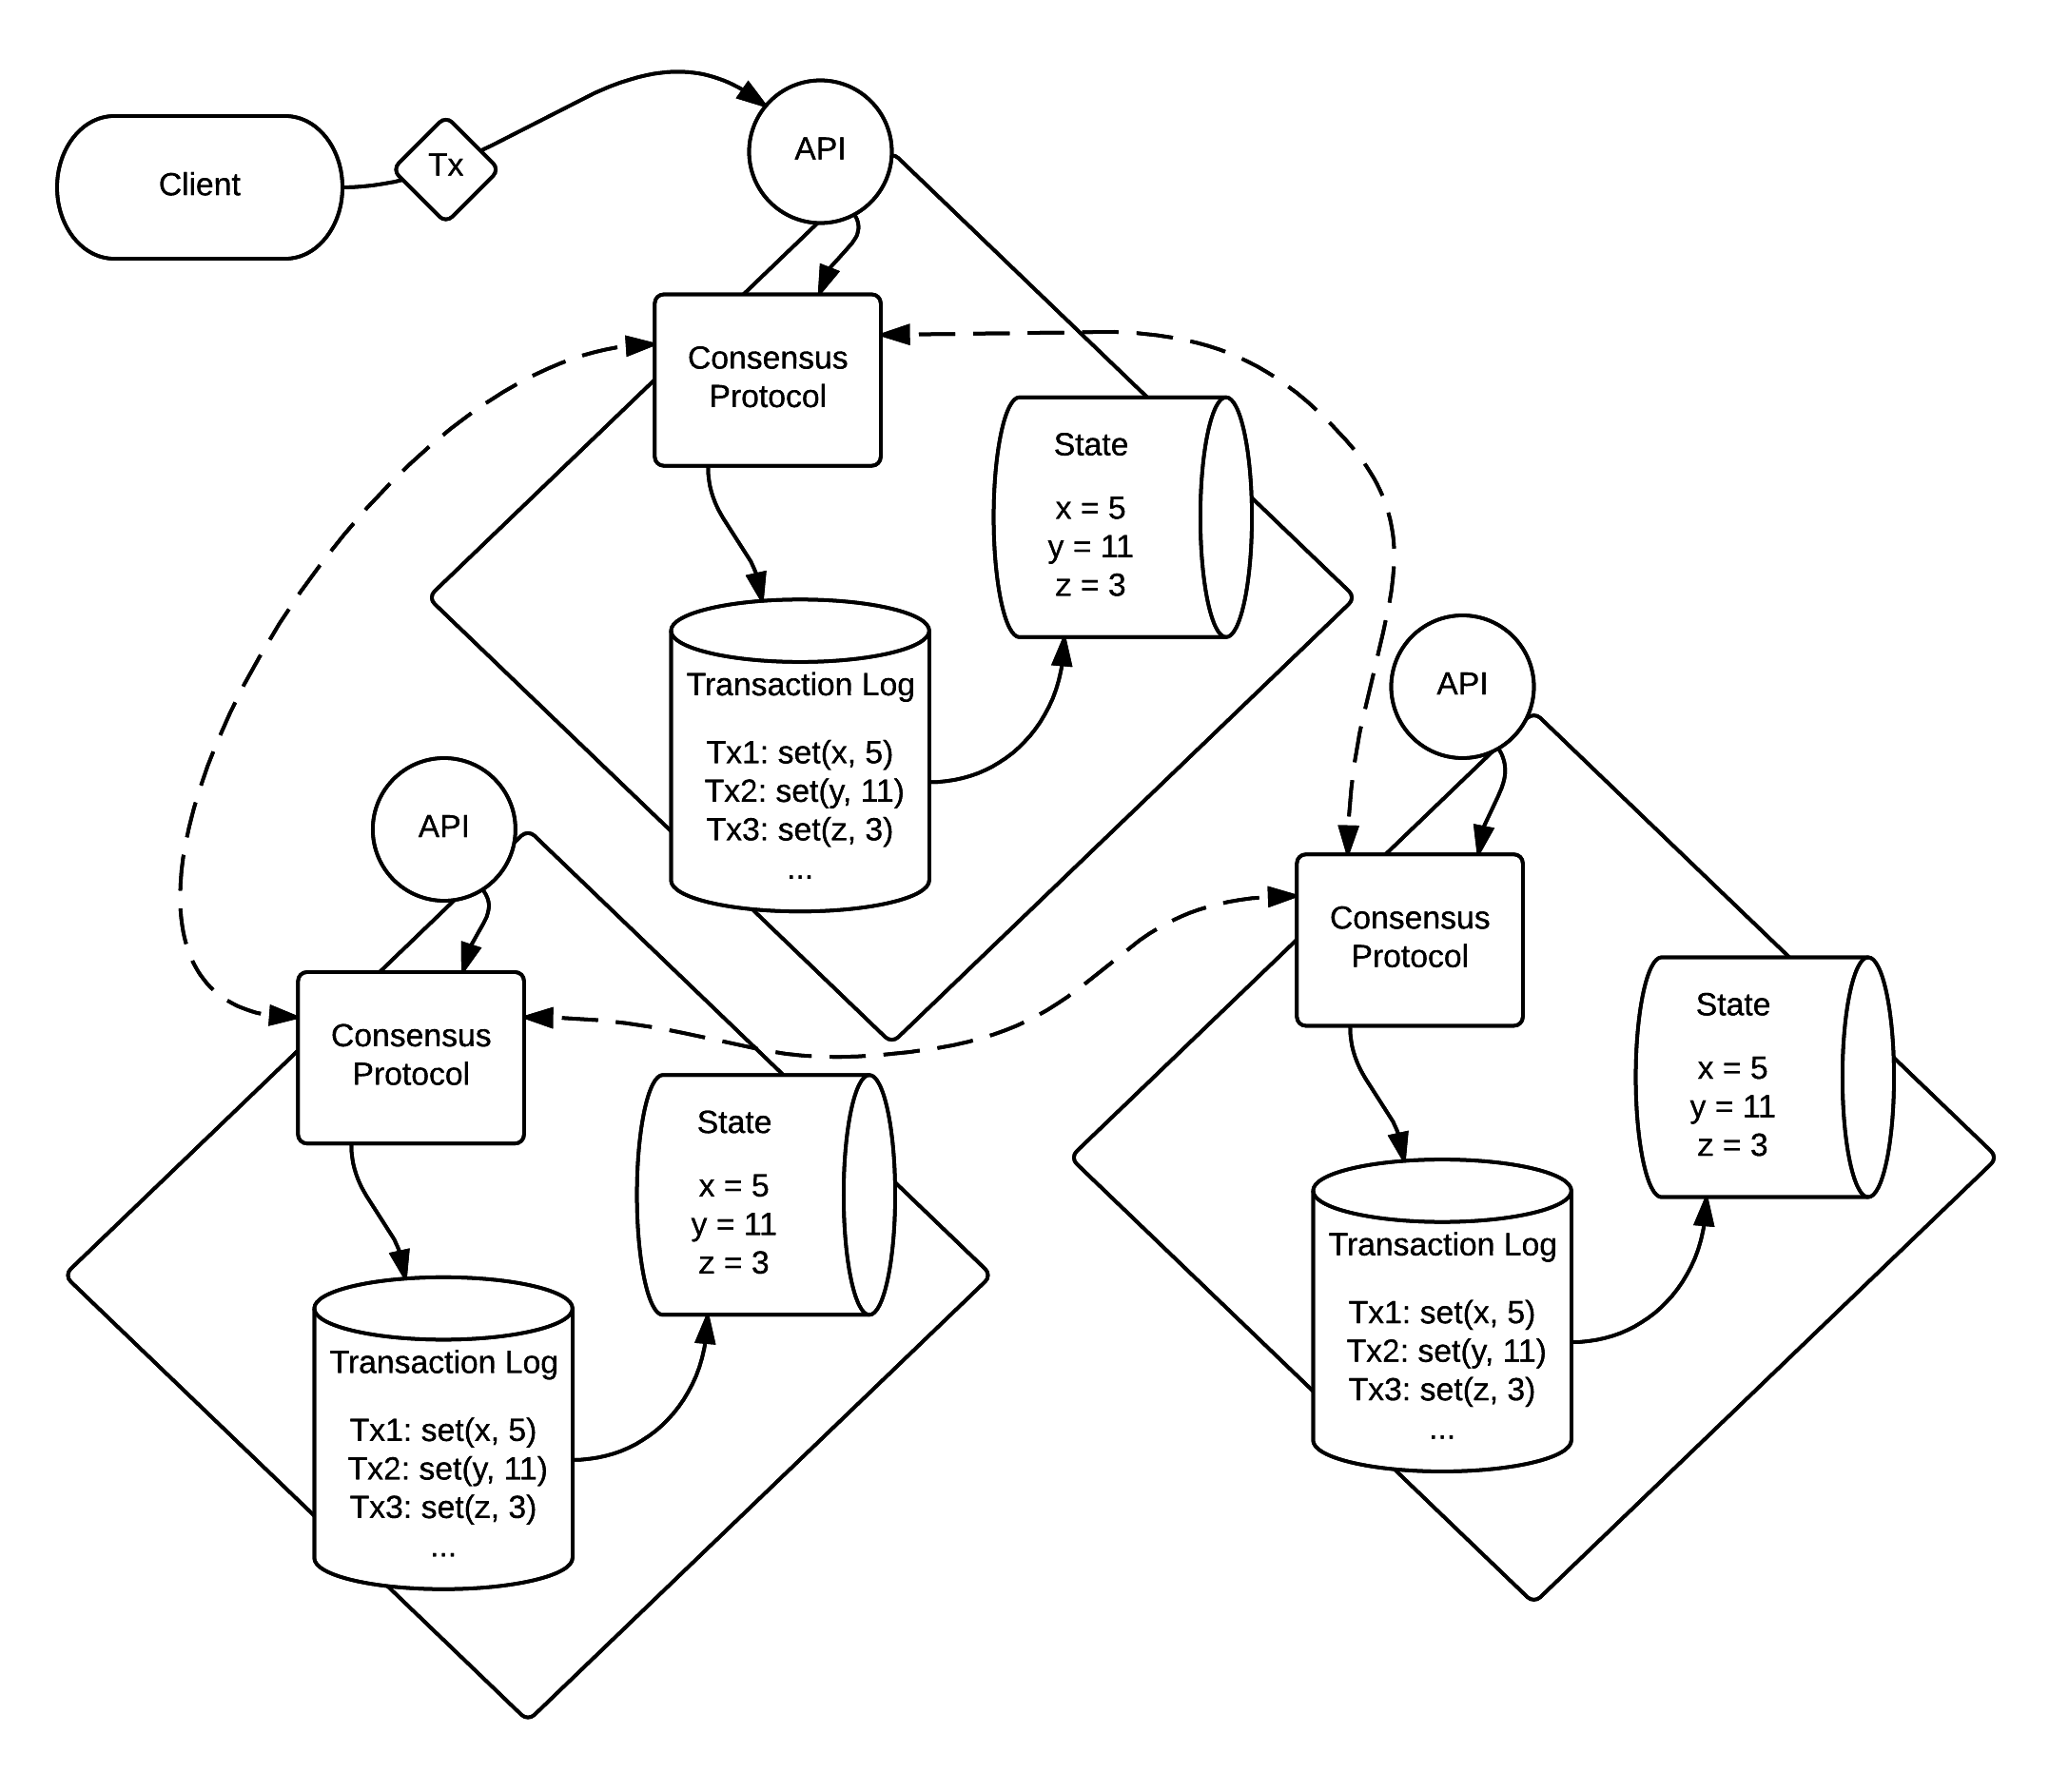
\includegraphics[width=\linewidth,height=\textheight,keepaspectratio]{figures/state_machine.png}
    	\centering
	\label{fig:replicated_state_machine}
	\caption[Overview of replicated state machine architecture]{
A replicated state machine replicates a transaction log and resulting state across multiple machines. 
Transactions are received from the client, 
run through the consensus protocol, 
ordered in the transaction log,
and executed against the state. 
In the figure, each diamond represents a single machine, 
with dotted lines representing communication between machines to carry out the consensus protocol for ordering transactions.}
\end{figure}

Tendermint was motivated from the desire to create a general purpose, high-performance, secure, and robust replicated state machine.

\section{Distributed Consensus}

The purpose of a fault-tolerant distributed consensus system is to co-ordinate a network of computers to 
stay in sync while providing a useful service, despite the presence of faults.
Staying in sync amounts to replicating the transaction log successfully; 
providing a useful service amounts to keeping the state machine available for new transactions.
These aspects of the system are traditionally known as \emph{safety} and \emph{liveness}, respectively.
Colloquially, safety means nothing bad happens; liveness means that something good eventually happens.
A violation of safety implies two or more valid, competing transaction logs.
Violating liveness implies an unresponsive network.

It is trivial to satisfy liveness by accepting all transactions. And it is trivial to satisfy safety by accepting none.
Hence, consensus algorithms can be seen to operate on a spectrum defined by these extremes.
Typically, nodes require some threshold of received information from other nodes before they commit a new transaction.
In synchronous environments, 
where we make assumptions about the maximum delay of network messages or the maximum speed of processor clocks,
 it is easy enough to take turns proposing new transactions, poll for a majority vote, 
and skip a proposer's turn if they don't propose within the bounds of the synchrony assumptions.

In asynchronous environments, where no such assumptions about network delays or processor speeds are warranted,
the trade-off is much more difficult to manage.
In fact, the so called FLP impossibility result demonstrates the 
impossibility of distributed consensus among deterministic asynchronous processes 
if even a single processes can crash\footnote{Prior to FLP, the distinction between sync/async wasn't as prominent}\cite{flp}.
The proof amounts to showing that, because processes can fail, 
there are valid executions of the protocol in which processes fail at the exact opportune times to prevent consensus.
Hence, we have no guarantee of consensus.

Typically, synchrony in a protocol is reflected by the use of timeouts to manage certain transitions.
In asynchronous environments, where messages can be arbitrarily delayed, relying on synchrony (timeouts) for safety
can lead to a fork in the transaction log.
Relying on synchrony to ensure liveness can cause the consensus to halt, and the service to become unresponsive.
The former case is usually considered more severe, as reconciling conflicting logs can be a daunting or impossible task. 

In the early 90s, Lamport broke new ground with the Paxos algorithm \cite{paxos},
which, while not fully asynchronous,
provided the first provably correct algorithm for distributed consensus in mostly asynchronous environments.
Paxos simultaneously empowered and confused the discipline of consensus science,
on the one hand by providing the first real-world, practical, fault-tolerant consensus algorithm,
and on the other by being so difficult to understand and explain.

Paxos became the staple consensus algorithm for industry, 
upon which the likes of Amazon \cite{dynamo}, Google \cite{chubby}, 
and others would build out highly available global internet services.
The Paxos consensus would sit at the bottom of the application stack, 
providing a consistent interface to resource management and allocation, 
operating at much slower time scales than the highly-available applications facing the users.
However, there has always been an understanding in the field that implementing Paxos is somewhat of a black art,
permeated by tricks for two main things: 
maintaining liveness in the face of asynchrony, and achieving consensus on more than one bit at a time.

Like most consensus algorithms before it, the official Paxos algorithm only achieves consensus on one bit at a time,
and involves an expensive leadership election process for each additional bit. 
Hence a variety of so called Multi-Paxos have been proposed, but no single approach dominates, 
and each implementation diverges in its own unique ways. 
The resulting software ecosystem is clumsy, difficult to navigate, and in some cases overly liable to contain bugs.
Some have worked to more more clearly define these difficulties 
and describe solutions \cite{chandra2007paxos}.

Seeking to remedy this situation, in 2013, Ongaro and Ousterhout published Raft \cite{raft},
an algorithm for consensus in asynchronous environments whose motivating design goal was understandability.
Raft is much simpler to understand than Paxos.
It has seen tremendous adoption in the open source community, 
with implementations in virtually ever major language \cite{raft.github.io},
and use as the backbone in major projects, 
including CoreOs's distributed Linux distribution \cite{coreos_raft} and the open source time-series database InfluxDB \cite{influxdb,hashicorp_raft}.

Raft's major divergent design decisions from Paxos was to focus on the transaction-log first, rather than a single bit,
and to allow a leader to persist in committing transactions until he goes down, 
at which point leadership election can kick in. 
In some ways, this is similar to the approach taken by blockchains, 
though the major advantage of blockchains is the ability to tolerate a different kind of fault.

\section{Byzantine Fault Tolerance}

Blockchains have been described as ``trust machines'' \cite{economist_blockchains} on account of the way they reduce counter party risk through the decentralization of responsibility over a shared database.
Bitcoin, in particular, is noted for its ability to withstand attacks and malicious behaviour by any of the participants. 
Traditionally, consensus protocols tolerant of malicious behaviour were known as Byzantine Fault Tolerant (BFT) consensus protocols.
The term Byzantine was used due to the similarity of the problem to that faced by generals of the Byzantine army attempting to co-ordinate themselves to attack Rome using only messengers,
where one of the generals may be a traitor \cite{lamport1982Byzantine}.

In a crash fault, a process simply halts. In a Byzantine fault, it can behave arbitrarily.
Crash faults are easier to handle, as no process can \emph{lie} to another process.
Systems which only tolerate crash faults can operate via simple majority rule, 
and therefore typically tolerate simultaneous failure of up to half of the system.
If the number of failures the system can tolerate is $f$, such systems must have at least $2f+1$ processes.

Byzantine failures are more complicated. In a system of $2f+1$ processes, if $f$ are Byzantine, 
they can co-ordinate to say arbitrary things to the other $f+1$ processes.
For instance, suppose we are trying to agree on the value of a single bit, 
and $f=1$, so we have $N=3$ processes, $A$, $B$, and $C$, where $C$ is Byzantine, as in Figure \ref{fig:byzantine}.
$C$ can tell $A$ that the value is $0$ and tell $B$ that it's $1$. 
If $A$ agrees that its $0$, and $B$ agrees that its $1$, then they will both think they have a majority and commit, 
thereby violating the safety condition.
Hence, the upper bound on faults tolerated by a Byzantine system is strictly lower than a non-Byzantine one.

\begin{figure}[]
	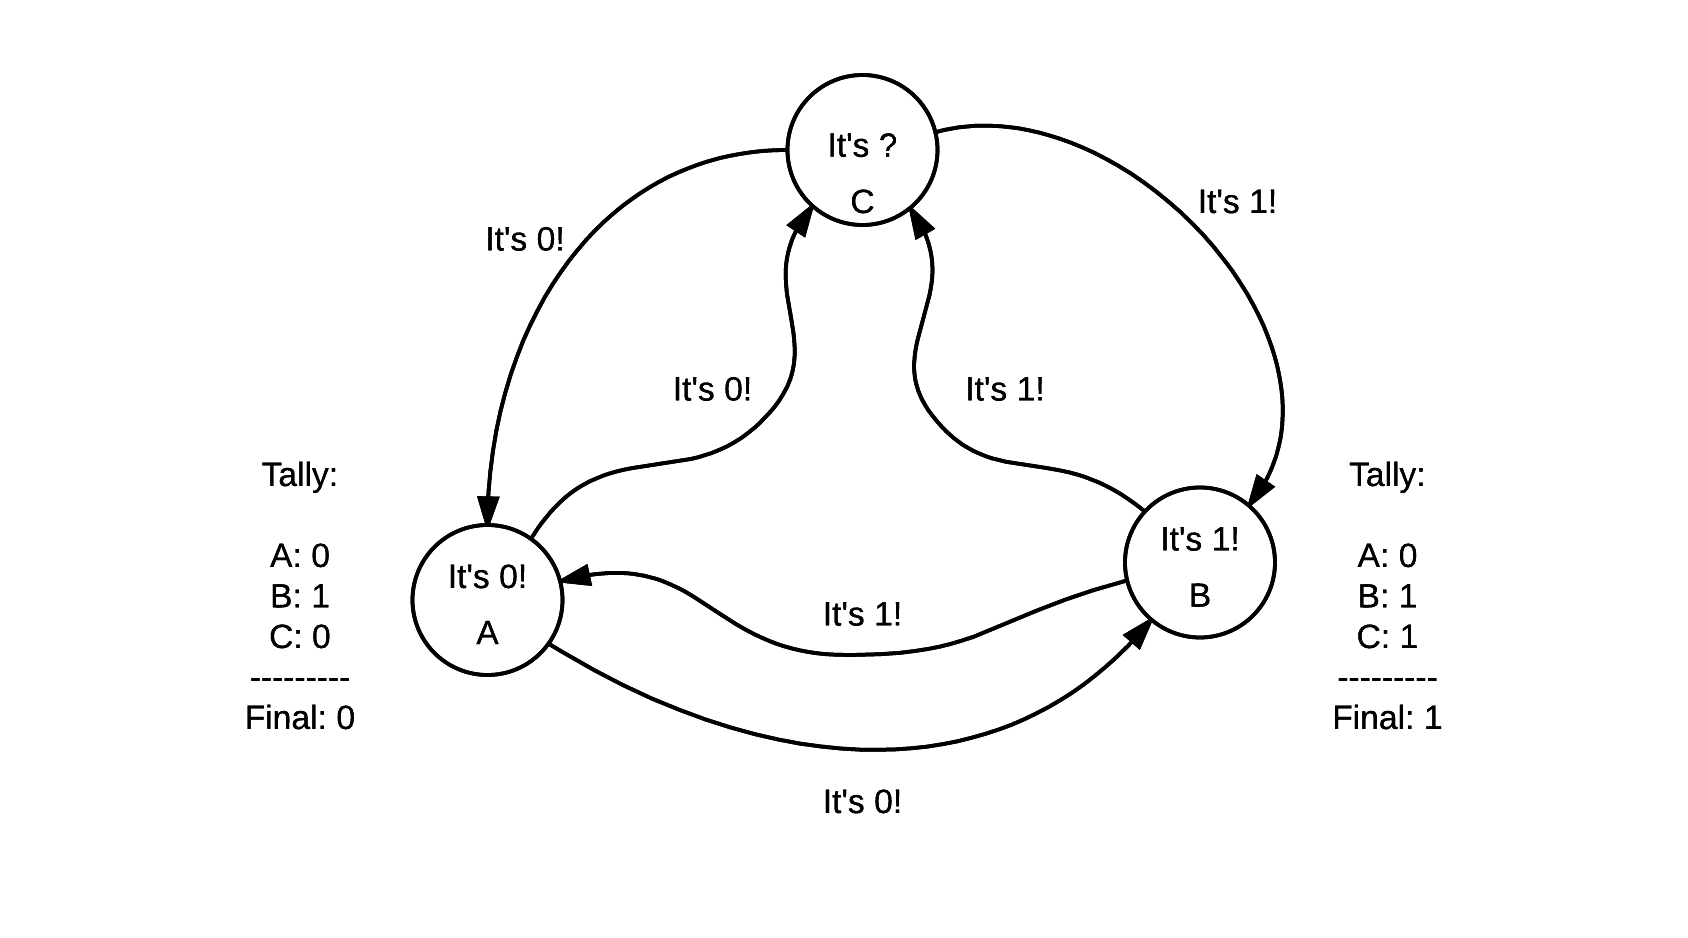
\includegraphics[width=\linewidth,height=\textheight,keepaspectratio]{figures/byzantine.png}
    	\centering
	\label{fig:byzantine}
	\caption[Byzantine nodes tell lies]{
A Byzantine node, C, tells A one thing and B another, causing them to come to different conclusions about the network.
Here, simple majority vote results in a violation of safety due to only a single Byzantine node.}
\end{figure}


In fact, it can be shown that the upper limit on $f$ for Byzantine faults is $f < N/3$ \cite{pease1980reaching}.
Thus, to tolerate a single Byzantine process, we require at least $N=4$. 
Then the faulty process can't split the vote the way it was able to when $N=3$.

In 1999, Castro and Liskov published Practical Byzantine Fault Tolerance \cite{pbft}, or \emph{PBFT}, 
which provided the first optimal Byzantine fault tolerant algorithm in asynchronous networks.
It set a new precedent for the practicality of Byzantine fault tolerance in industrial systems by being capable 
of processing tens of thousands of transactions per second.
Despite this success, Byzantine fault tolerance was still considered expensive and largely unnecessary, 
and the most popular implementation was difficult to build on top of \cite{ppbft}.
Hence, despite a resurgence in academic interest, including numerous improved variations \cite{yin2003separating, kotla2007zyzzyva}
not much progress was made in the way of implementations and deployment.
Furthermore, PBFT provides no guarantees in the face of a complete Byzantine failure, where a third or more of the network is malicious.

\section{The Need For Tendermint}

The success of Bitcoin and its derivatives, especially Ethereum, and their promise of secure, autonomous, distributed, fault-tolerant execution of arbitrary code has caused virtually every major financial institution on the planet to start paying attention to the blockchain phenomenon. 
In particular, there has emerged an understanding of two forms of the technology:
On the one hand are the public blockchains, known affectionately as the Big Bad Public Blockchains or BBPBs, 
whose protocols are dominated by in-built economic incentives bootstrapped by a native currency.
On the other are so called private blockchains, which might more accurately be called ``consortia blockchains'',
and which are effectively improvements on traditional consensus and BFT algorithms through the use of hash trees, digital signatures, 
peer-to-peer networking, and enhanced accountability.

As the infrastructure of our societies continues to decentralize, and as the nature of business becomes more inter-organizational,
there is increasing need for a transparent, accountable, high performance BFT system, which can support applications from finance to domain registration to electronic voting,
and which comes equipped with advanced mechanisms for governance and evolution into the future.
Tendermint is that solution, optimized for consortia, or inter-organizational logic, but flexible enough to accommodate anyone from private enterprise to global currency,
and high-performance enough to compete with the major, non-BFT, consensus solutions available today, such as etcd, consul, and zookeeper, while providing greater resilience, security guarantees, and flexibility to application developers.

A more comprehensive discussion of consensus science and related algorithms is reserved for Chapter \ref{ch:related}


\chapter{Tendermint Consensus}
\label{ch:tendermint}

This chapter presentes the Tendermint consensus algorithm and communicates the intuitions underlying its security.

\section{Tendermint Overview}

Tendermint consensus is an algorithm for the secure replication of a state machine that operates on batches, or blocks, of transactions at a time.
The algorithm is summarized in \ref{fig:tendermint_summary}, it's key properties as a replicated state machine are summarized in \ref{fig:tendermint_gaurantees}, and its key security properties are summarized in \ref{fig:tendermint_security}.

\begin{figure}[]
	\underline{Consensus State}
		\begin{description}
			\item[ValidatorSet:] ordered list of validators. There is at most one valid proposer for every term.
			\item[LastCommit:] set of $+\frac{2}{3}$ precommits for last block. Empty for first block.
			\item[Height:] strictly increasing from 0. One unique block per height.
			\item[Round:] resets to zero at each height. Accommodates asynchrony. 
			\item[Proposal:] signed proposal of block to commit at next height.
			\item[VoteSet:] set of votes from validators on proposals (or nil) for any round at the current height.
			\item[LockedBlock:] last block precommitted.
			\item[LockedRound:] first round the LockedBlock was precommitted by this validator.
		\end{description}

	\underline{Proposal Message}
		\begin{description}
			\item[Broadcast by next proposer in round-robin.]
			\item[Only one valid proposer (and message) at each round.]
			\item[Arguments:] Height, Round, BlockHash, Signature
		\end{description}

	\underline{Vote Message}
		\begin{description}
			\item[Broadcast by validators in response to proposals and other votes.]
			\item[Two types: prevote and precommit.]
			\item[Arguments:] Height, Round, Type, BlockHash, Signature
		\end{description}

	\caption[Summary of tendermint protocol]{Summary of data types in the tendermint protocol}
	\label{fig:tendermint_summary}
\end{figure}


\begin{figure}[]
	\underline{Consensus State Rules}
		\begin{description}
			\item[Proposal:] Wait up to TimeoutPropose for a proposal from the correct validator for the current height and round.
			\item[Prevote:]  If a proposal comes with a valid signature from the correct proposer for a validator’s current height and round, and the validator is not locked, it should prevote for the proposal block. Else, prevote nil.
			\item[Precommit:] If a validator receives prevotes from $+\frac{2}{3}$ validators for the same block, it should precommit for that block. If the $+\frac{2}{3}$ prevotes are not for the same block, it should wait TimeoutPrevote, and then precommit nil.
			\item[Commit:] If a validator receives precommits from $+\frac{2}{3}$ validators for the same block, it should commit that block, and go to the next height.  If the $+\frac{2}{3}$ prevotes are not for the same block, it should wait TimeoutPrecommit, and then go to the next round.
		\end{description}

	\underline{Broadcast Rules}
		\begin{description}
			\item[No Double Signing:] a validator only signs for each message type (proposal, prevote, precommit) once at a given height and round.
			\item[Prevote The Lock:] A validator is locked on the last block they precommitted, and must prevote for that block in future rounds at that height.
			\item[Unlock On Polka:] a validator may only unlock if there have been $+\frac{2}{3}$ prevotes at a round after they locked. 
		\end{description}
		Violation of any of the Broadcast Rules is detectable and should be punished.

	\caption[Summary of tendermint protocol rules]{Summary of rules in the tendermint protocol}
	\label{fig:tendermint_summary}
\end{figure}




\begin{figure}[]
	\textbf{Tendermint Safety Guarantees}
	\begin{description}
	  \item[Proposer Safety] \hfill \\
		There is at most one valid proposer for every term.
	  \item[Validator Append Only] \hfill \\
		A validator never overwrites or deletes blocks it has committed.
	  \item[Block Matching] \hfill \\
		If two validators contain a block at the same height, it is the same block.
	  \item[Proposer Completeness] \hfill \\
		If a block is committed at a given height, then that block will be present in the chain of all proposers at greater heights.
	  \item[State Machine Safety] \hfill \\
		If a validator has applied a block at a given height to its state machine, no other validator will ever apply a different block for the same height.
	\end{description}
  	\caption[Tendermint Safety Guarantees]{Tendermint gaurantees that all of these properties are true, at all times, within the security gaurantee. This set of properties was taken practically verbatim from \cite{raft_thesis}}
	\label{fig:tendermint_gaurantees}
\end{figure}

\begin{figure}[]
	\textbf{Tendermint Security Guarantees}
	\begin{description}
	  \item[Byzantine Fault Tolerance] \hfill \\
		All properties in \ref{fig:tendermint_gaurantees} are satisfied so long as fewer than one-third of validators are Byzantine
	  \item[Deterministic Accountability] \hfill \\
		If one-third or more of validators, but less than half, are Byzantine, and thereby compromise safety, 
		they can be specifically identified and held accountable to their actions.
	\end{description}
  	\caption[Tendermint Security Guarantees]{Tendermint gaurantees these security properties, making it more suitable than algorithms like Raft and Paxos, and even other BFT algorithms like PBFT, for consortia with potentially malicious or untrusted actors}
	\label{fig:tendermint_security}
\end{figure}


Consensus begins with a set of \emph{validators}, each of which is responsible for maintaining a full copy of the replicated state,
and for participating in consensus by proposing and voting on new blocks (batches of transactions).
Each block is assigned an incrementing index, or \emph{height}, such that a valid blockchain has only one valid block at each height.
At each height, validators take turns proposing new blocks in \emph{rounds}, such that for any given round there is at most one valid proposer.
It may take multiple rounds to commit a block at a given height due to the asynchrony of the network,
and the network may halt altogether if more than one-third of the validators are offline or partitioned.
Validators engage in two phases of voting on a proposed block before it is committed, 
and follow a simple locking mechanism which prevents any coalition of up to one third malicious validators from compromising safety.

Each block contains some metadata, known as its \emph{header}, which includes the hash of the block at the previous height, resulting in a hash chain.
The header also includes the block height, local time the block was proposed, and the merkle root hash of transactions included in the block.

The consensus algorithm can be roughly divided into the following, somewhat orthogonal, components:

\begin{itemize}

\item{Proposals: a new block must be proposed by the correct proposer at each round, and gossipped to the other validators. If a proposal is not received in sufficient time, the proposer should be skipped}

\item{Votes: two phases of voting must occur to ensure optimal Byzantine fault tolerance. They are called \emph{pre-vote} and \emph{pre-commit}. A set of pre-commits from more than two-thirds of the validators for the same block at the same round is a \emph{commit}.}

\item{Locks: Tendermint ensures that no two validators commit a different block at the same height, presuming less than one-third of the validators are malicious. This is achieved using a locking mechanism which determines how a validator may pre-vote or pre-commit depending on previous pre-votes and pre-commits at the same height. Note that this locking mechanism must be carefully designed so as to not compromise liveness.}

\end{itemize}

As will be seen, Tendermint affords an ability to identify and hold accountable malicious validators, thus providing greater security gaurantees than competing algorithms.

\section{Why Blocks?}

Tendermint is designed specifically to work with batches, or blocks, of transactions at a time.
Most consensus algorithms commit transactions one at a time by design, and implement batching after the fact.
Using blocks results in two primary optimizations, which give us more throughput and fault-tolerance:

\begin{itemize}
\item{Bandwidth optimization: since every commit requires two rounds of communication across all validators, 
	batching transactions in blocks amortizes the cost of a commit over all the transactions in the block.}
\item{Integrity optimization: the hash chain of blocks forms an immutable data structure, much like a git repository, enabling authenticity checks for sub-states at any point in the history}
\end{itemize}

Blocks induce another effect as well, which is more subtle but potentially important. 
They increase the minimum latency of a transaction to that of the whole block, which for tendermint is on the order of hundreds of milliseconds to seconds.
Traditional serializable database systems provide commit latencies on the order of milliseconds to tens of milliseconds.
They are able to do this because they are not Byzantine Fault Tolerant, requiring only one round of communication (instead of two)
and responses from over half of the replicas (instead of two-thirds).
However, unlike the fast commit times interupted by leader elections in other consensus algorithms,
Tendermint provides a more regular pulse that is more responsive to the overall health of the network, in terms of node failures and asynchrony.

What role such pulses might play in the coherence of communicating autonomous systems on the internet is yet to be determined.

\section{Tendermint Basics}

In order to provide tolerance to a single Byzantine fault, a Tendermint network must contain at minimum four validators.
Each validator must possess an assymetric cryptographic key-pair for producing digital signatures.
Validators start from a common \emph{genesis} state, which contains the initial list of validators in terms of their public keys.
All proposals and votes must be signed by the respective validator's private key, and can hence be verified by every other validator.
It is helpful to assume that up to one-third of validators are malicious, co-operating in arbitrary ways to subvert system safety or liveness.

Consensus begins for block 1, round 0; the proposer is the first validator listed in the genesis.
The outcome of a round is either a commit, or a decision to move to the next round.
With a new round comes the next proposer.
Using multiple rounds gives validators multiple opportunties to come to consensus in the event of network asynchrony or validator failures.

In contrast to algorithms which require a form of leader election, Tendermint has a new leader (the proposer) for each round.
Validators vote to skip to the next round in the same way they vote to accept the proposal,
lending the protocol a uniniformity of mechanism that is absent from algorithms with an explicit leader-election program.

The beginning of each round has a weak dependence on synchrony as it utilizes local clocks to determine when to skip a proposer.
That is, if a validator does not receive a proposal within a locally measured \emph{TimeoutPropose} of entering a new round, it can vote to skip the proposer.
Inherent in this mechanism is the assumption that, at least eventually, the proposal will be delivered within TimeoutPropose, which may itself increment with each round.
This assumption is discussed more fully later (TODO).

After the proposal, rounds proceed in a fully asynchronous manner - a validator makes progress only after hearing from more than two-thirds of the other validators.
This relieves any sort of dependence on synchronized clocks or bounded network delays,
but implies that the network will halt if one-third or more of the nodes become unresponsive.

To round-skip safely, a small number of \emph{locking} rules are introduced which force validators to justify their votes.
While we don't necessarily require them to broadcast their justifications in real time, we do expect them to keep the data,
such that it can be brought forth as evidence in the event a total Byzantine failure.
This accountability mechanism enables Tendermint to provide stronger gaurantees in the face of such failure than eg. PBFT,
which provides no gaurantees if a third or more of validators are Byzantine.

Validators communicate using a diverse set of messages for managing the blockchain, application state, peer network, and consensus.
The core consensus algorithm, however, consists of just two messages:

\begin{itemize}
\item{ProposalMsg: a proposal for a block at a given height and round, signed by the proposer}
\item{VoteMsg: a signed vote for a proposal}
\end{itemize}

In practice, we use additional messages to optimize the gossiping of block data and votes, as discussed in Chapter \ref{ch:subprotocols}

\section{Proposals}

Each round begins with a proposal. 
The propser for the given round takes a batch of recently received transactions from its local cache (the Mempool, see Chapter \ref{ch:subprotocols}),
composes a block, and broadcasts a signed ProposalMsg containing the block.
If the proposer is Byzantine, it might broadcast different proposals to different validators.

Proposers are ordered via a simple, deterministic round robin, 
so only a single proposer is valid for a given round, 
and every validator knows the correct proposer. 
If a proposal is received for a lower round, or from an incorrect proposer, it is rejected.

Cycling of proposers is necessary for Byzantine tolerance. 
For instance, in Raft, if an elected leader is Byzantine and maintatins strong network connections to other nodes,
it can completely compromise the system, destroying all safety and liveness gaurantees.
Tendermint preserves safety via the voting and locking mechanisms, 
and maintains liveness by cycling proposers, so if one won't process any transactions, others can pick up.
Perhaps more interestingly, validators can vote through governance modules (see LATER) to remove or replace Byzantine validators.

\iffalse
TODO: move the tuning comment 
Upon entering a new round, validators wait ProposalTimeout to receive a complete proposal before broadcasting their pre-vote.
The ProposalTimeout thus serves as a critical paramter for tuning the performance of the system,
as it determines how much latency is permitted from proposers before validators start voting to skip them.
\fi

\section{Votes}

Once a complete proposal is received by a validator, 
it signs a pre-vote for that proposal and broadcasts it to the network.
If a validator does not receive a correct proposal within ProposalTimeout, 
it signs and broadcasts a \emph{nil-pre-vote} instead.

In Byzantine environments, a single stage of voting is not sufficient to ensure safety.
This can be seen via a proof by contradcition.
Suppose that a single round of voting, where more than two-thirds vote for a single block, were sufficient to commit the block.
Consider a network with validators Val1, Val2, Val3, and Val4, where Val1 is Byzantine.
Suppose Val1 both votes for the proposal, and nil-votes (it is Byzantine).
Suppose Val2 and Val3 vote, while Val4 nil-votes (it didn't receive the proposal in time).
Now, suppose Val2 sees the pre-votes from Val1, itself, and Val3, and hence commits the proposed block,
but Val3 and Val4 only see messages from eachother and the nil-prevote from Val1.
Now Val3 and Val4 go to the next round, while Val2 has already committed, and only Val1 is Byzantine.
Val1 also goes to the next round and the three of them commit a block.
Now Val2 has committed one block while Val3 and Val4 have committed another while less than one-third of the validators (only Val1) are Byzantine,
thus violating safety. 

The importance of the example is to illustrate why using only a single round of voting
is not sufficient if some validators can be Byzantine.
A single round of voting allows validators to tell eachother what they know about the proposal.	
But to tolerate Byzantine faults (which amounts, essentially to lies, fraud, deceipt, etc.), 
they must also tell eachother what they know about what other validators have professed to know about the proposal.

Thus, pre-voting is a preparation phase, in which validators synthesize what other validators know.
A pre-vote for a block is a vote to prepare the network to commit the block.
A nil-pre-vote is a vote to prepare the network to move to the next round.
In an ideal round with an online proposer, more than two-thirds of validators will pre-vote for the proposal.
A set of more than two-thirds of pre-votes for a single block at a given round is known as a \emph{polka} \footnote{The original term used was PoL, or PoLC, for Proof-of-Lock or Proof-of-Lock-Change, as discussed LATER. The term evolved to polka as it was realized the validators are doing the polka}.
A set of more than two-thirds of pre-votes for nil is a \emph{nil-polka}

When a validator recieves a polka (read: more than two-thirds pre-votes for a single block), 
it signals that the network is prepared to commit the block,
and serves as justification for the validator to sign and broadcast a pre-commit vote for that block.
Sometimes, due to network asynchrony, a validator may not receive a polka, or there may not have been one. 
In that case, the validator is not justified in signing a pre-commit for that block, 
and must therefore sign and publish a pre-commit vote for nil (nil-pre-commit).
That is, it is considered malicious behaviour to sign a pre-commit without justification from a polka.

A pre-commit is a vote to actually commit a block.
A nil-pre-commit is a vote to actually move to the next round.
If a validator receives more than two-thirds pre-commits for a single block, 
it commits that block, computes the resulting state,
and moves on to round 0 at the next height.
If a validator receives more than two-thirds nil-pre-commits,
it moves on to the next round.

\section{Locks}

Ensuring safety across rounds can be tricky, 
as circumstances must be avoided which would provide justification for two different blocks to be committed at two different rounds at the same height, 
In Tendermint, this problem is solved via a \emph{locking} mechanism.
In essence, once a pre-commit is cast, a validator is \emph{locked} on the associated block, and must follow certain locking rules.
There are three rules of locking:

\begin{itemize}
\item{Prevote-the-Lock: a validator must pre-vote for the block they are locked on. 
	This prevents validators from pre-committing one block in one round, 
	and then contributing to a polka for a different block in the next round, 
	thereby compromising safety.}
\item{Release-Lock-on-Polka: a validator may only release a lock after seeing a polka or nil-polka at a round greater than that at which it locked.
	This allows validators to unlock if they pre-committed something the rest of the network doesn't want to commit,
	thereby protecting liveness, but does it in a way that does not compromise safety,
	by only allowing unlocking if there has been a polka in a round after that in which the validator became locked.}
\end{itemize}


For simplicity, a validator is considered to have locked on nil at round -1 at each height, so that Release-Lock-on-Polka implies that a validator cannot precommit at all at a new height until they see a polka.

These rules can be understood more intuitively by way of examples. 
Consider again our four validators, and suppose there is a proposal for $blockA$ at round $R$. 
Suppose there is a polka for $blockA$, but Val1 doesn't see it, and precommits nil, while the others precommit for $blockA$.
Now suppose the only one to see all precommits is Val4, while the others, say, don't see Val4's precommit (they only see their two precommits and Val1's nil-precommit).
Val4 will now commit the block, while the others go to round $R+1$.
Since any of the validators might be the new proposer, if they can propose any new block, say $blockB$, then they might commit it and compromise safety, since Val4 already committed $blockA$.
Note that there isn't even any Byzantine behaviour here, just asynchrony!

Locking solves the problem by forcing validators to stick with the block they pre-committed, since other valdiators might have committed based on those precommits (as Val4 did).
In essence, once more than two-thirds precommit a block in a round, the network is locked on that block,
which is to say it must be impossible to produce a valid polka for a different block at a higher round.
This is direct motivation for Prevote-the-Lock.

Prevote-the-Lock is not sufficient, however. There must be a way to unlock, lest we sacrifice liveness.
Consider a round where Val1 and Val2 precommitted $blockA$ while Val3 and Val4 precommitted nil.
They all move to the next round, and $blockB$ is proposed, which Val3 and Val4 prevote for.
Suppose Val1 is Byzantine, and prevotes for $blockB$ as well (despite being locked on $blockA$), resulting in a polka.
Suppose Val2 does not see the polka and precommits nil, while Val1 goes off-line and Val3 and Val4 precommit $blockB$. 
They move to the next round, but Val2 is still locked on $blockA$, while Val3 and Val4 are now locked on $blockB$, 
and since Val1 is offline, they can never get a polka. Hence, we've compromised liveness with less than a third (here, only one) Byzantine validators.

The obvious justification for unlocking is a polka. Once Val2 sees the polka for $blockB$ (which Val3 and Val4 used to jusitfy their precommits for $blockB$), 
it ought to be able to unlock, and hence precommit $blockB$.

...

\section{Safety}

- Proposer Safety condition implied by protocol
- Validator Append Only condition implied by the protocol
- Proposer Completeness guaranteed by the merkle hash chain

Need to show Block Matching, State Machine Safety, and Deterministic Accountability.
Locking rules give us lemmas about polkas.





\section{Faults and Availability}

As a BFT consensus algorithm, Tendermint can tolerate Byzantine failure in up to (but not including) one-third of validators.
This means nodes can crash, send different and contradictory messages to different peers, refuse to relay messages, or otherwise behave arbitrarily,
without compromising safety or liveness (with the usual FLP caveat for liveness).

There are two places in the protocol where we can make optimizations for asynchrony by utilizing timeouts based on local clocks:
after receiving two-thirds or more pre-votes, but not for a single block or nil, and after receiving two-thirds or more pre-commits, 
but not for a single block or nil.
In each case, we can sleep for some amount of time to give slower or delayed votes a chance to be received,
thereby reducing the likelihood of going to a new round without committing a block.
Clocks do not need to be synced across validators, as they are reset each time a validator observes votes from two-thirds or more others.

If a third or more of validators crash, the network halts, 
as no validator is able to make progress without hearing from two-thirds or more of the validator set.
The network remains available for reads, but no new commits can be made.
As soon as validators come back on-line, they can carry on from where they left in a round. 
The consensus state-machine should employ a write-ahead log (see LATER),
such that a recovered validator can quickly return to the step it was in when it crashed.

If a third or more of validators are Byzantine, they can compromise safety a number of ways, 
for instance by proposing two blocks for the same round, and voting both of them through to commit, 
or by pre-committing on two different blocks at the same height but in different rounds by violating the rules on locking.
In each case, there is clear, identifiable evidence that certain validators misbehaved. 
In the first instance, they signed two proposals at the same round, a clear violation of the rules.
In the second, they may have pre-voted for a different block in round $R$ than they locked on in $R-1$, 
a violation of the Prevote-the-Lock rule.

When using economic and governance components to incentivize and manage the consensus (see LATER), 
these additional accountability gaurantees become critical.

\section{Conclusion}

Tendermint is Awesome.




\chapter{Tendermint Subprotocols}
\label{ch:subprotocols}

The presentation of Tendermint consensus in the previous chapter left out a number of details
regarding the gossip protocols used to disseminate blocks, votes, transactions, 
and other peer information. 
This was done in order to focus in on the consensus protocol itself, 
without distraction from the hydra of practical software engineering.
This chapter describes one particular approach to filling in these details,
by implementing components as relatively independent reactors that are multiplexed over each peer connection.

\section{P2P-Networking}

On startup, each Tendermint node receives an initial list of peers to dial.
For each peer, a node maintains a persistent TCP connection over which multiple subprotocols are multiplexed in a rate-limited fashion.
Messages are serialized into a compact binary representation to be sent on the wire, and 
connections are encrypted via an authenticated encryption protocol \cite{authenticated_encryption}.

Each remaining section of this chapter describes a separate reactor that is multiplexed over each peer connection.
An additional peer exchange reactor can be run which allows nodes to request other peer addresses from each other and keep track of peers they have connected to before,
in order to stay connected to some minimum number of other peers.

\section{Consensus Gossip}

The consensus reactor wraps the consensus state machine, 
and ensures each node broadcasts to all peers its current state every time it changes.
In this way, each node keeps track of the consensus state of all its peers, 
allowing it to optimize the gossiping of messages to only send peers information they need at the very moment,
and which they don't already have.
For each peer, a node maintains two routines which continuously check for new information to send the peer,
namely, proposals and votes. 
Information should be gossiped in a ``rarest first'' manner in order to maximize 
gossip efficiency and minimize the chance that some information becomes unavailable \cite{rarest_first}


\subsection{Block Data}
In Chapter \ref{ch:tendermint}, it was assumed that proposal messages include the block.
However, since blocks emerge from a single source and can be quite large, 
this puts undue pressure on the block proposer to upload the data to all other nodes;
blocks can be disseminated much more quickly if they are split into parts and gossiped.

A common approach to securely gossiping data, as popularized by various p2p protocols \cite{bittorrent,libswift}, 
is to use a Merkle tree \cite{merkle1987digital},
allowing each piece of the data to be accompanied by a short proof (logarithmic in the size of the data)
that the piece is a part of the whole. 
To use this approach, 
blocks are serialized and split into chunks of an appropriate size 
for the expected block size and number of validators,
and chunks are hashed into a Merkle tree. 
The signed proposal, instead of including the entire block, includes just the Merkle root hash,
allowing the network to co-operate in gossiping the chunks.
A node informs its peers every time it receives a chunk, 
in order to minimize the bandwidth wasted by transmitting the same chunk to a node more than once.

Once all the chunks are received, the block is deserialized and validated to ensure it refers correctly to the previous 
block, and that its various checksums, implemented as Merkle trees, are correct. 
While it was previously assumed that a validator does not pre-vote until the proposal (including the block) is received,
some performance benefit may be obtained by allowing validators to pre-vote after receiving a proposal, 
but before receiving the full block. This would imply that it is okay to pre-vote for what turns out to be an invalid block.
However, pre-committing for an invalid block must always be considered Byzantine.

Peers that are catching up (i.e.~are on an earlier height) are sent chunks for the height they are on,
and progress one block at a time.

\subsection{Votes}

At each step in the consensus state machine, after the proposal, a node is waiting for votes (or a local timeout) to progress.
If a peer has just entered a new height, it is sent pre-commits from the previous block,
so it may include them in the next blocks \emph{LastCommit} if it's a proposer.
If a peer has pre-voted but has yet to pre-commit, or has pre-committed, but has yet to go to the next round,
it is sent pre-votes or pre-commits, respectively.
If a peer is catching up, it is sent the pre-commits for the committed block at its current height.

\section{Mempool}

Chapter \ref{ch:tendermint} made little mention of transactions, 
despite the purpose of a consensus algorithm being to order and execute transactions,
as Tendermint operates on blocks on a time, and has no concern for individual transactions,
so long as their checksum in the block is correct.

Transactions are managed independently in an in-memory cache, 
which, following Bitcoin, has come to be known as the \emph{mempool}.
Transactions are validated by the application logic when they are received and, if valid, 
added to the mempool and gossiped using an ordered multicast algorithm.
A node maintains a routine for each peer which ensures that transactions 
in the mempool are sent to the peer in the same order in which they were processed by the node.

Proposers reap transactions from the ordered list in the mempool for new block proposals.
Once a block is committed, all transactions included in the block are removed from the mempool,
and the remaining transactions are re-validated by the application logic,
as their validity may have changed on account of other transactions being committed, 
which the node may not have had in its mempool.

\section{Syncing the Blockchain}

The consensus reactor provides a relatively slow means of syncing with the latest state of the blockchain,
as it was designed for real-time consensus,
meaning peers wait to receive all information to commit a single block before worrying about the next block.
To accommodate peers that may be more than just a few blocks behind, 
an additional reactor, the blockchain reactor, allows peers to download many blocks in parallel,
enabling a peer to sync hundreds of times faster than via the consensus reactor.

When a node connects to a new peer, the peer sends its current height.
The node will request blocks, in order, beginning with its current height,
from all peers that self-reported higher heights, and download the blocks concurrently, adding them to the block pool.
Another routine continuously attempts to remove blocks from the pool and add them to the blockchain by validating and executing them, 
two blocks at a time, against the latest state of the blockchain.
Blocks must be validated two blocks at a time because the commit for one block is included as the LastCommit data in the next one.

The node continuously queries its peers for their current height, 
and continues to concurrently request blocks until it has caught up to the highest height among its peers, 
at which point it stops making requests for peer heights and starts the consensus reactor.


\chapter{Building Applications}
\label{ch:apps}

Tendermint is designed to be a general purpose algorithm for replicating a deterministic state machine.
It uses the Tendermint Socket Protocol (TMSP) to standardize communication between the consensus engine and the state machine,
enabling application developers to build their state machines in any programming language, 
and have it automatically replicated via Tendermint's BFT algorithm.

\section{Background}

Applications on the internet can in general be characterized as containing two fundamental components:

\begin{itemize}
\item{Engine: handles core security, networking, replication. 
This is typically a webserver, like Apache or Nginx, when powering a web app, 
or a consensus algorithm when powering a distributed application.}
\item{State-machine: the actual application logic that processes transactions received from the engine and updates internal state.}
\end{itemize}

This separation of concerns enables application developers to write state-machines in any programming language representing arbitrary applications,
on top of an engine which may be specialized for its performance, security, usability, support, and other considerations.

Unlike web-servers and their applications, which often take the form of processes communicating over a socket via the Common Gateway Interface (CGI) protocol,
consensus algorithms have traditionally had much less usable or less general purpose interfaces to build applications on top of.
Some, like zookeeper, etcd, consul, and other distributed key-value stores, 
provide HTTP interfaces to a particular instance of a simple key-value application, 
with some more interesting features like atomic compare-and-swap operations and push notifications.
But they do not give the application developer control of the state-machine code itself.

Demand for such a high-level of control over the state-machine running above a consensus engine has been driven primarily by the success of Bitcoin and the consequent interest in blockchain technology.
By building more advanced applications directly into the consensus, 
users, developers, regulators, etc.~can achieve greater security guarantees on arbitrary state-machines, 
far beyond key-value stores, like currencies, exchanges, supply-chain management, governance, and so on.
What has captured the attention of so many is the potential of a system which permits collective enforcement of the execution of code.
It is practically a re-invention of many dimensions of the legal system, using distributed consensus algorithms and deterministically executable contracts,
rather than policemen, lawyers, judges, juries, and the like.
The ramifications for the development of human society are explosive, much as the introduction of the democratic rule of law was in the first place.

Tendermint aims to provide the fundamental interface and consensus engine upon which such applications might be built.

\section{Tendermint Socket Protocol}

The Tendermint Socket Protocol (TMSP) defines the core interface by which the consensus engine communicates with the application state machine.
The interface definition consists of a number of message types, specified using Google's Protocol Buffers \cite{protobuf}, 
that are length-prefixed and transmitted over a socket. 
A list of message types, their arguments, return values, and purpose is given in Figure \ref{fig:tmsp_msgs},
and an overview of the architecture and message flow is shown in Figure \ref{fig:tmsp}.

\begin{figure}[]
\vspace*{-1.5in}
    	\centering
\begin{verbatim}

type Application interface {
	// Return application info
	Info() (info string)

	// Set application option
	SetOption(key string, value string) (log string)

	// Append a tx
	AppendTx(tx []byte) Result

	// Validate a tx for the mempool
	CheckTx(tx []byte) Result

	// Return the application Merkle root hash
	Commit() Result

	// Query for state
	Query(query []byte) Result

	// Signals the beginning of a block
	BeginBlock(height uint64) 

	// Signals the end of a block
	// validators: changed validators from app to TendermintCore
	EndBlock(height uint64) (validators []*Validator)
}

type CodeType int32

type Result struct {
	Code CodeType
	Data []byte
	Log  string // Can be non-deterministic
}

type Validator struct {
	PubKey []byte 
	Power  uint64 
}
\end{verbatim}
	\caption[TMSP Message Types]{
The TMSP application interface as defined in Golang.
TMSP messages are defined using Google's Protocol Buffers, and their serialized form is length prefixed before 
being sent over the TMSP socket. 
Return values include a \emph{Code}, similar to an HTTP Status Code, representing any errors,
and $0$ is used to indicate no error.
Messages are buffered client side until a \emph{Flush} message is sent,
at which point all messages are transmitted. While the server design is asynchronous, message responses must be correctly ordered and match their request.
}
	\label{fig:tmsp_msgs}
\end{figure}


\begin{figure}[]
	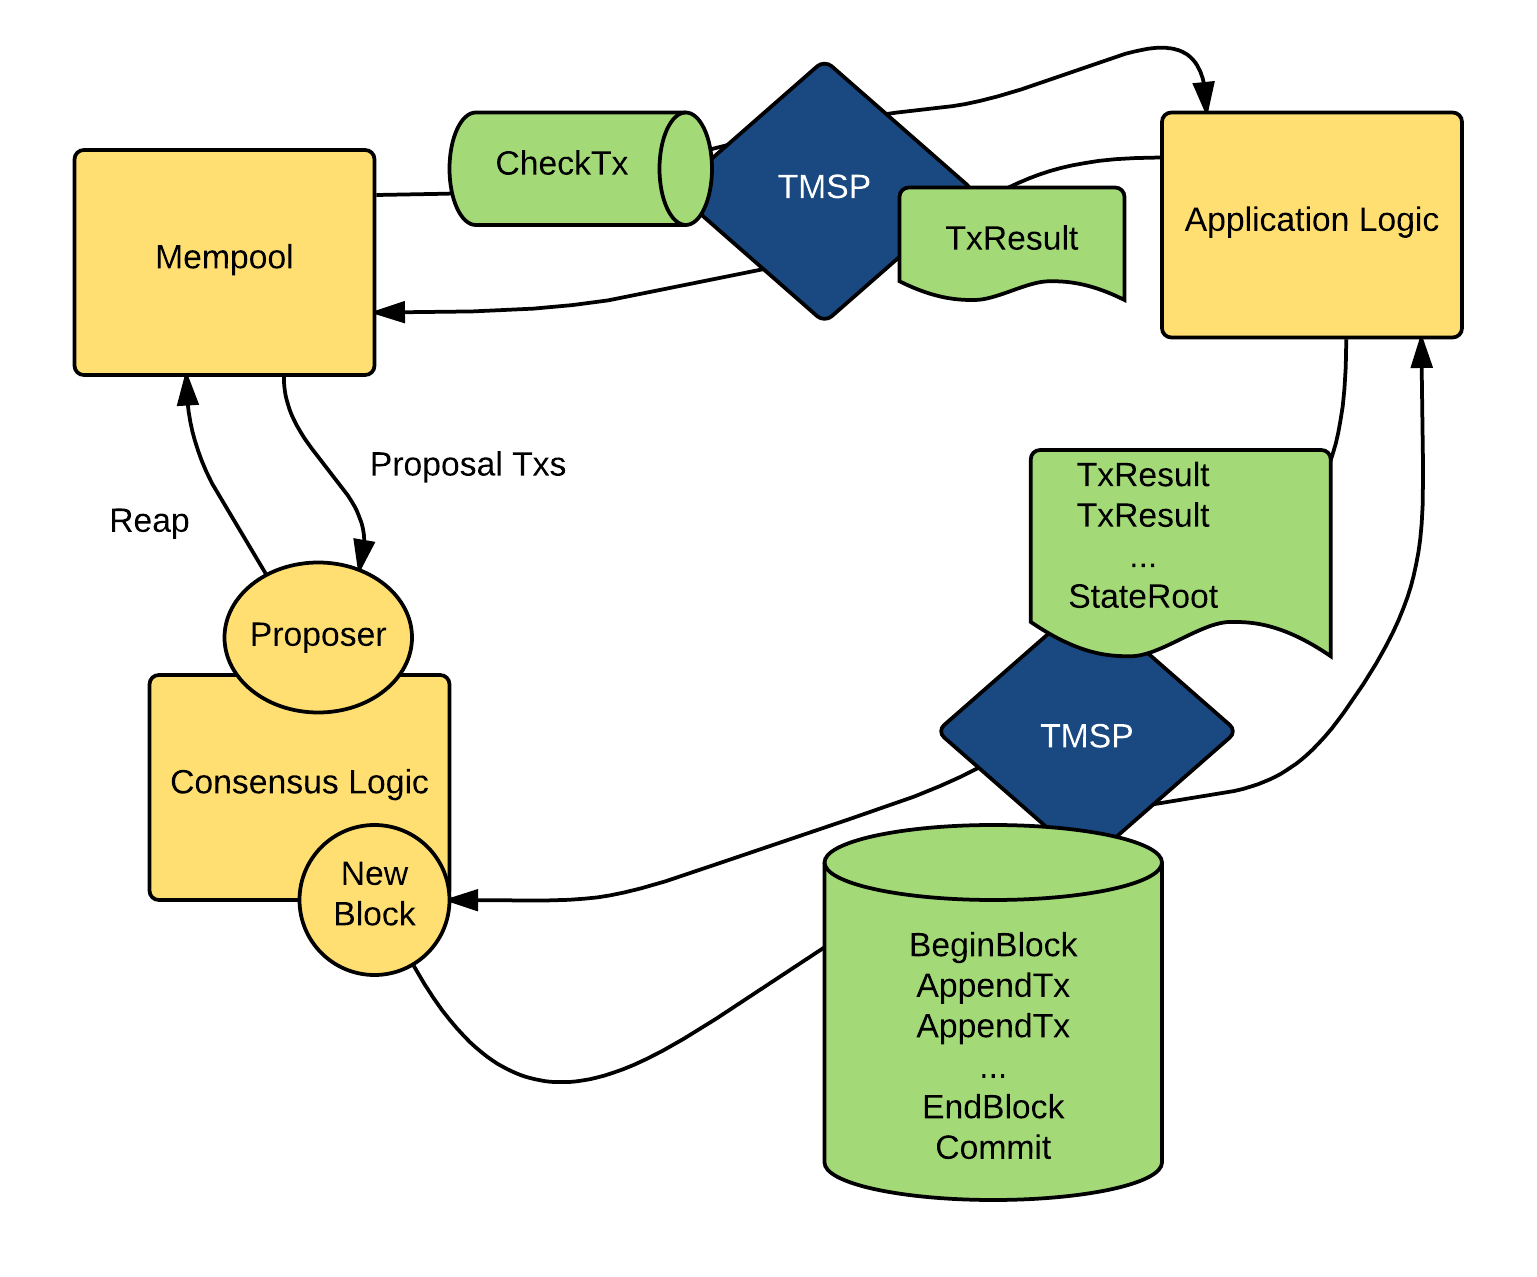
\includegraphics[width=\linewidth,height=\textheight,keepaspectratio]{figures/diagrams/tmsp.png}
    	\centering
	\caption[TMSP Architecture]{
The consensus logic communicates with the application logic via TMSP, a socket protocol. 
Two sockets are maintained, one for the mempool to check the validity of new transactions,
and one for the consensus to execute newly committed blocks.
}
	\label{fig:tmsp}
\end{figure}

TMSP is implemented as an ordered, asynchronous server, 
where message types come in pairs of request and response,
and where a special message type, Flush, pushes any buffered messages over the connection and awaits all responses.

At the core of the TMSP are two messages: \emph{AppendTx} and \emph{Commit}.
Once a block is decided by the consensus, 
the engine calls \emph{AppendTx} on each transaction in the block, 
passing it to the application state-machine to be processed.
If the transaction is valid, it will result in a state-transition in the application.

Once all \emph{AppendTx} calls have returned, the consensus engine calls Commit,
causing the application to commit to the latest state, and persist it to disk.

\section{Separating Agreement and Execution}

Using the TMSP affords us an explicit separation between consensus, or agreement on the order of transactions, 
and their actual execution in the state-machine.
In particular, we achieve consensus on the order first, and then execute the ordered transactions.
This separation actually improves the system's fault tolerance \cite{yin2003separating}:
while $3f+1$ replicas are still needed for agreement to tolerate $f$ Byzantine failures, 
only $2f+1$ replicas are needed for execution.
That is, while we still need a two-thirds majority for ordering, we only need a one-half majority for execution.

On the other hand, the fact that transactions are executed after they are ordered results in possibly invalid transactions,
which can waste system resources. 
This is solved using an additional TMSP message, \emph{CheckTx}, which is called by the mempool,
allowing it to check whether the transaction would be valid against the latest state.
Note, however, that the fact that commits come in blocks at a time introduces complexity in the handling of \emph{CheckTx} messages.
In particular, applications are expected to maintain a second state-machine that executes only those rules of the main state-machine pertaining to a transaction's validity. 
This second state-machine is updated by \emph{CheckTx} messages and is reset to the latest committed state after every commit.
In essence, the second state machine describes the transaction pool's filter rules.

To some extent, \emph{CheckTx} can be used as an \emph{optimistic execution} \cite{optimistic_execution},
returning a result to the transaction sender with the caveat that 
the result may be wrong if a block is committed with a conflicting transaction
before the transaction of interest is committed.
This sort of optimistic execution is the focus of an approach to scalable BFT systems 
that can work quite well for particular applications where conflicts between transactions are rare. 
At the same time, it adds additional complexity to the client, by virtue of needing to handle possibly invalid results.
The approach is discussed further in Chapter \ref{ch:related}.

\section{Microservice Architecture}

Adopting separation of concerns as a strategy in application design is generally considered wise practice \cite{hursch1995separation}.
In particular, many large scale application deployments today adopt a microservice architecture,
wherein each functional component is implemented as a standalone network service, 
and typically encapsulated in a linux container (e.g.~using Docker) for efficient deployment, scalability, and upgradeability.

Applications running above Tendermint consensus will often be decomposable into microservices.
For instance, many applications will utilize a key-value store for storing state.
Running the key-value store as an independent service is quite common, 
in order to take advantage of the data store's specialized features, such as high-performance data types or Merklization.

Another important microservice for applications is a governance module, 
which manages a certain subset of TMSP messages, enabling the application to control validator set changes.
Such a module can become a powerful paradigm for governance in BFT systems.

Some applications may utilize a native currency or account structure for users.
It may thus be useful to provide a module which supports basic elements of, for instance,
handling digital signatures and managing account dynamics.

The list of possible microservices to compose a complex TMSP application goes on. 
In fact, one might even build an application which can launch sub-applications using data sent in transactions.
For instance, including the hash of a docker image in a transaction,
such that the image could be pulled from some file-storage backend and run as a sub-application where
future transactions in the consensus could cause it to execute. 
This is the approach of ethereum, 
which allows developers to deploy bits of code to the network that can be triggered to run within the Ethereum Virtual Machine by future transactions \cite{ethereum},
and of IBM's recent OpenBlockChain (OBC) project, which allows developers to send full docker contexts in transactions, 
defining containers that run arbitrary code in response to transactions addressed to them \cite{obc}.

\section{Determinism}

The most critical caveat about building applications using TMSP is that they must be deterministic.
That is, for the replicated state-machine to not compromise safety, 
every node must obtain the same result when executing the same transaction against the same state.

This is not a unique requirement for Tendermint. Bitcoin, Raft, Ethereum, any other distributed consensus algorithm,
and applications like lock-step multiplayer gaming must all be strictly deterministic, lest a consensus failure arise.

There are many sources of non-determinism in programming languages, most obviously via random numbers and time,
but also, for instance, via the use of floating point precision, and by iteration over hash tables 
(some languages, such as Go, enforce randomized iteration over hash tables to force programmers to be explicit about when they need ordered data structures).
The strict restriction on determinism, and its notable lacking from every major programming language,
prompted ethereum to develop its own, Turing-complete, fully deterministic virtual machine,
which forms the platform for application developers to build applications above the ethereum blockchain.
While deterministic, it has many quirks, such as 32-byte stack words, storage keys, and storage values,
and no support for byte-shifting operations - everything is big number arithmetic.

Deterministic programming is well studied in the world of real-time, lockstep, multi-party gaming.
Such games constitute another example of replicated state machines, and are quite similar in many ways to consensus algorithms.
Application developers building with TMSP are encouraged to study their methods, and to take care when implementing an application.
On the one hand, the use of functional programming languages and proof methods can enable the construction of correct programs.
On the other, compilers are being built to translate possibly non-deterministic programs to canonically deterministic ones \cite{deterministicjs}.

\section{Termination}

If determinism is critical for preserving safety, termination of transaction execution is critical for preserving liveness.
It is, however, not in general possible to determine whether a given program halts for even a single input, let alone all of them,
a problem known as the Halting Problem \cite{halting, davis1958computability}.

Ethereum's virtual machine solves the problem by \emph{metering}, that is, charging for each operation in the execution.
This way, a transaction is guaranteed to terminate when the sender runs out of funds.
Such metering may be possible in a more general case, 
via compilers that compile programs to metered versions of themselves.

It is difficult to solve this problem without significant overhead.
In essence, a validator cannot tell if an execution is in an infinite loop or is just slow, but nearly complete.
It may be possible to use the Tendermint consensus protocol to decide on transaction timeouts, 
such that more than two-thirds of validators must agree that a transaction timed out and is thus considered invalid (ie. having no effect on the state).
However, we do not pursue the idea further here, leaving it to future work. 
In the meantime, it is expected that applications will undergo thorogh testing before being deployed in any consensus system,
and that monitoring and governance mechanisms will be used to resurrect the system in the event of consensus failure.

\section{Examples}

In this section, examples of increasingly more complex TMSP applications are introduced and discussed,
with particular focus on \emph{CheckTx} and managing the mempool.

\subsection{Merkleeyes}

A simple example of a TMSP application is a Merklized key-value store. 
Tendermint provides Merkleeyes, a TMSP application which wraps a self-balancing, Merkle binary search tree.
The first byte of a transaction determines if the transation is a get, set, or remove operation. 
For get and remove operations, the remaining bytes are the key. 
For the set operation, the remaining bytes are a serialized list containing the key and value.
Merkleeyes may utilize a simple implementation of \emph{CheckTx} that only decodes the transaction,
to ensure it is properly formatted.
One could also make a more advanced \emph{CheckTx}, where get and remove operations on unknown keys are invalid.
Once Commit is called, the latest updates are added into the Merkle tree, all hashes are computed, 
and the latest state of the tree is committed to disk.

Note that Merkleeyes was designed to be a module used by other TMSP applications for a Merklized key-value store,
rather than a stand alone TMSP application, though the simplicity of the TMSP interface makes it amenable to both.

\subsection{Basecoin}

A more complete example is a simple currency, 
using an account structure pioneered by Ethereum, 
where each user has a public key and an account with the balance for that public key.
The account also contains a sequence number, which is equal to the number of transactions sent by the account.
Transactions can send funds from the account if they include the correct sequence number
and are signed by the correct private key.
Without the sequence number, the system would be susceptible to replay attacks \cite{replay},
where a signed transaction debiting an account could be replayed, 
causing the debit to occur multiple times.
Furthermore, to prevent replay attacks in a multi-chain environment, 
transaction signatures should include a network or blockchain identifier.

An application supporting a currency has naturally more logic than a simple key-value store.
In particular, certain transactions are distinctly invalid, 
such as those with an invalid signature, incorrect sequence number,
or sending an amount greater than the sender's account balance.
These conditions can be checked in \emph{CheckTx}.

Furthermore, a supplementary application state must be maintained for \emph{CheckTx} 
in order to update sequence numbers and account balances 
when there are multiple transactions involving the same accounts in the mempool at once.
When commit is called, the supplementary application state is reset to the latest committed state.
Any transactions still in the mempool can be replayed via \emph{CheckTx} against the latest state.

\subsection{Ethereum}

Ethereum uses the mechanisms already described to filter transactions out of the mempool,
but it also runs some transactions in a virtual machine, 
which updates state and returns results.
The virtual machine execution is not done in \emph{CheckTx}, 
as it is much more expensive and depends heavily on the ultimate order of transactions as they are included in blocks.

\section{Conclusion}

TMSP provides a simple yet flexible means to build arbitrary applications,
in any programming language,
that inherit BFT state-machine replication from the Tendermint consensus algorithm.
It plays much the same role for a consensus engine and an application that, for instance, CGI plays for Apache and Wordpress.
However, application developers must take special care to ensure their applications are deterministic, and that transaction executions terminate.


\chapter{Governance}
\label{ch:governance}

So far, this thesis has reviewed the basic elements of the Tendermint consensus protocol and application environment.
Critical elements of operating the system in the real world, such as managing validator set changes
and recovering from crisis, have not yet been discussed. 

This chapter proposes an approach to these problems that formalizes the role of governance in a consensus system.
As validator sets come to encompass more decentralized sets of agents, competent governance systems 
for maintaining the network will be increasingly paramount to the network's success.

\section{Governmint}

The basic functionality of governance is to filter proposals for action, typically through a form of voting.
The most basic implementation of governance as software is a module that enables users to make proposals,
vote on them, and tally the votes. 
Proposals may be programmatic, in which case they may execute automatically following a successful vote,
or they may be non-programmatic, in which case their execution is a manual excercise.

To enable certain actions in Tendermint, such as changing the validator set or upgrading the software,
a governance module has been implemented, called Governmint.
Governmint is a minimum viable governance application with support for multiple groups of entities,
each of which can vote internally on proposals, some of which may result in programmatic execution of actions,
like changing the validator set, or upgrading governmint itself (for instance to add new proposal types or other voting mechanisms).

The system utilizes digital signatures to authenticate voters, 
and may use a variety of possible voting schemes.
Of particular interest are quadratic voting schemes,
where the cost to vote is quadratic in the weight of the vote,
which have been shown to have a superior ability to satisfy voter preferences \cite{posner2013quadratic}.

\section{Validator Set Changes}

Validator set changes are a critical component of real world consensus algorithms that many previous approaches have failed to specify 
or have been left as a black art. 
Raft took pains to expound a sound protocol for validator set changes which required the change pass through consensus, 
using a new message type.
Tendermint takes a similar approach, though it is standardized through the TMSP interface using the \emph{EndBlock} message,
which is run after all the \emph{AppendTx} messages, but before \emph{Commit}.
If a transaction, or set of transactions, is included in a block with the intended effect of updating the validator set,
the application can return a list of validators to update by specifying their public key and new voting power 
in response to the \emph{EndBlock} message.
Validators can be removed by setting their voting power to zero.
This provides a generic means for applications to update the validator set without having to specify transaction types.

If the block at height $H$ returns an updated validator set, 
then the block at height $H+1$ will reflect the update.
Note, however, that the \emph{LastValidation} in block $H+1$
must utilize the validator set as it was at $H$, 
since it may contain signatures from a validator that was removed.

Changes to voting power are applied for $H+1$ such that the next proposer 
is effected by the update. 
In particular, the validator that otherwise should have been the next proposer may be removed.
The round robin algorithm should handle this gracefully, simply moving on to the next proposer in line.
Since the same block is replicated on at least two-thirds of validators, 
and the round robin is deterministic,
they will all make the same update and expect the same next proposer.

\section{Punishing Byzantine Validators}

One of the salient points of Bitcoin's design is its incentive comptability, 
in so far as the goal of the protocol was to incentivize validators to behave correctly
by rewarding them. While this makes sense in the context of Bitcoin's conensus protocol,
a superior incentive may be to provide strong dis-incentives, such that validators
have real \emph{skin-in-the-game} \cite{taleb2014skin}, rather than a soft opportunity cost.

Disincentives can be achieved in Tendermint using an approach first proposed by Vitalik Buterin \cite{slasher} as a so-called Proof-of-Stake protocol.
In essence, validators must make a security deposit (``they must bond some stake'')
in order to participate in consensus.
In the event that they are found to double-sign proposals or votes, 
other validators can publish evidence of the transgression in the form of a transaction, 
which the application state can use to change the validator set by removing the transgressor, burning its deposit.
This has the effect of associating an explicit economic cost with Byzantine behaviour, 
and enables one to estimate the cost of violating safety by bribing a third or more of the validators to be Byzantine.

Note that a consensus protocol may specify more behaviours to be punished than just double signing.
In particular, we are interested in punishing any strong signalling behaviour which is unjustified - typically, any reported change in state that is not based on the reported state of others.
For instance, in a version of Tendermint where all precommits 
must come with the polka that justifies them,
validators may be punished for broadcasting unjustified precommits.
Note, however, that we cannot just punish for any unexpected behaviour - 
for instance, a validator proposing when it is not their round to propose
may be a basis for optimizations which pre-empt asynchrony or crashed nodes.

In fact, a generalization of Tendermint along these two lines, 
of 1) looser forms of justification and 2) allowing validators to propose before their term,
gives rise to a family of protocols similar in nature to that proposed by Vlad Zamfir,
under the guise Casper, as the consensus mechanism for a future version of ethereum \cite{casper}.
A more formal account of the relationship between the protocols, 
and of the characteristics of anti-Byzantine justifications, remains for future work.

\section{Software Upgrades}

Governmint can also be used as a natural means for negotiating software upgrades on a possibly decentralized network.
Software upgrades on the public internet are a notoriously challenging operation,
requiring careful planning to maintain backwards compatibility for users that don't upgrade right away,
and to not upset loyal users of the software by introducing bugs, removing features, adding complexity, or,
perhaps worst of all, updating automatically without permission.

The challenge of upgrading a decentralized consensus system is made especially apparent with Bitcoin.
While Ethereum has already managed a successful, non-backwards-compatible upgrade, 
due to its strong leadership and unified community,
Bitcoin has been unable to make some needed upgrades,
despite a plethora of software engineering ills,
on account of the a viciously divided community and a lack of strong leadership.

Upgrades to blockchains are typically differentiated as being \emph{soft forks} or \emph{hard forks},
on account of the scope of the changes.
Soft forks are meant to be backwards compatible, and to use degrees of freedom in the protocol that may be ignored
by users who have not upgraded, but which provide new features to users which do.
Hard forks, on the other hand, are non-backwards compatible upgrades that,
in Bitcoin's case, may cause violations of safety, 

and in Tendermint's case, cause the system to halt.

To cope, developers of the Bitcoin software have rolled out a series of softforks which validators can vote for
by signalling in new blocks. 
Once a certain threshold of validators are signalling for the update,
it automatically takes effect across the network, at least for users with a version of the software supporting the update.
The utility of the Bitcoin system has grown tremendously on account of these softforks, 
and is exepected to continue to do so on account of upcoming ones.
Interestingly, the failure of the community to successfully hard fork the software has
on the one hand raised concerns about the long term stability of the system,
and on the other triggered excitement and inspiration about the system's resilience to corrupt governance - its ungovernability.

While there are many reasons to take the latter stance, 
given the overwhelming government corruption apparent in the world today,
cryptography and distributed consensus provide a new set of tools that enables a degree
of transparency and accountability otherwise not imaginable in the paper-pen-handshake world of modern governments,
nor even the digital world of the traditional web, which suffers tremendously from sufficiently robust authentication systems.

In a system using Governmint, developers would be identifiable entities on the blockchain,
and may submit proposals for software upgrades. 
The mechanic is quite similar to that of a Pull Request on Github, 
only it is integrated into a live running system,
and the agreement passes through the consensus protocol.
Clients should be written with configurable update parameters, 
so they can specify whether to update automatically or to require they are notified first.

Of course, any software upgrade which is not thoroughly vetted could pose a danger to the system,
and a conservative approach to upgrades should be taken in general.

\section{Crisis Recovery}

In the event of a crisis, such as a fork in the transaction log,
or the system coming to a halt, 
a traditional consensus system provides little or no guarantees,
and typically requires manual intervention.

Tendermint assures that those responsible for violating safety can be identified,
such that any client who can access at least one honest validator 
can discern with cryptographic certainty who the dishonest validators are,
and thereby chose to follow the honest validators onto a new chain with a validator set excluding those who were Byzantine.

For instance, suppose a third or more validators violate locking rules,
causing two blocks to be committed at height $H$.
The honest validators can determine who double-signed by gossipping all the votes.
At this point, they cannot use the consensus protocol, because the basic fault assumptions have been violated.
One approach is for each validator to wait until they have all 
Note that being able to at this point accumulate all votes for $H$ 
implies strong assumptions about network connectivity and availability during the crisis,
which, if it cannot be provided by the p2p network, may require validators use alternative means, 
such as social media and high availability services, to communicate evidence.
A new blockchain can be started by the full set of remaining honest nodes, 
once at least two-thirds of them have gathered all the evidence.

Alternatively, modifying the Tendermint protocol so that precommits require polka
would ensure that those responsible for the fork could be punished immediately,
and would not require an additional publishing period. 
This modification remains for future work.

More complex uses of Governmint are possible for accomodating various particularities of crisis,
such as permanent crash failures and the compromise of private keys.
However, such approaches must be carefully thought out, 
as they may undermine the safety guarantees of the underlying protocol.
We leave investigation of these methods to future work, 
other than to note the importance of the socio-economic context a blockchain is embedded in to understand its ability to recover from crisis.

Regardless of how crisis recovery proceeds, its success depends on integration with clients.
If clients do not accept the new blockchain, the service is effectively offline.
Thus, clients must be aware of the rules used by the particular blockchain to recover.
In the cases of safety violation described above, they must also gather the evidence,
determine which validators to remove, and compute the new state with the remaining validators.
In the case of the liveness violation, they must keep up with Governmint.

\section{Conclusion}

Governance is a critical element of a distributed consensus system, 
though competent governance systems remain poorly understood.
Tendermint provides governance as a TMSP module called Governmint,
which aims to facilitate increased experimentation in software-based governance for distributed systems.


\chapter{Client Considerations}

This chapter reviews some considerations pertaining to clients that interact with an application hosted on Tendermint.

\section{Discovery}

Network discovery occurs simply by dialing some set of seed nodes over tcp.
The p2p network uses authenticated encryption, but the public keys of the validators must be verified somehow out of band.
Indeed, in these systems, the genesis state itself must be communicated out of band, and ideally is the only thing that must be communicated, 
as it should also contain the public keys used by validators for authenticated encryption, 
which are different than those used for signing votes in consensus.

For validator sets that may change over time, it is useful to register all validators via DNS, 
and to register new validators before they actually become validators, and remove them after they are removed as validators.
Alternatively, validator locations can be registered in another fault-tolerant distribtued data store, 
including possibly another Tendermint cluster itself.

\section{Broadcasting Transactions}

As a generalized application platform, tendermint provides only a simple interface to clients for broadcasting transaction.
The general paradigm is that a client connects to a Tendermint consensus network through a proxy, which is either run locally on its machine,
or hosted by some other provider. The proxy functions as a non-validator node on the network, 
which means it keeps up with the consensus and processes transactions, but does not sign votes.
The proxy enables client transactions to be quickly broadcast to the whole network via the gossip layer.

A node need only connect to one other node on the network to broadcast transactions, but by default will connect to many,
minimizing the chances that the transaction will not be received.
Transactions are passed into the mempool, 
and gossipped through the mempool reactor to be cached in the mempool of all nodes, 
so that eventually one of them will include it in a block. 

Note that the transaction does not execute against the state until it gets into a block,
so the client does not get a result back right away, other than confirmation that it was accepted into the mempool and broadcast to other peers.
Clients should register with the proxy to receive the result as a push notification when it is computed during the commit of a block.

It is not essential that a client connect to the current proposer, 
as eventually any validator which has the transaction in its mempool may propose it.
However, preferential broadcasting to the next proposer in line may lead to lower latency for the transaction
in certain cases where the network is under high load. Otherwise, the transaction should be quickly gossiped to every validator.

\section{Mempool}

The mempool is responsible for caching transactions in memory before they are included in blocks.
It's behaviour is subtle, and forms a number of challenges for the overall system architecture.
First and foremost, caching arbitrary numbers of transactions in the mempool is a direct denial of service attack
that could trivially cripple the network. Most blockchains solve this problem using their native currency,
and permitting only transactions which spend a certain fee to reside in the mempool.

In a more generalized system, like Tendermint, where there is not necessarily a currency to pay fees with,
the system must establish stricter filtering rules and rely on more intelligent clients to resubmit transactions that are dropped.
The situation is even more subtle, however, because the ruleset for filtering transactions in the mempool must be a function of the application itself.
Thus, TMSP includes an additional message type, CheckTx, 
which the mempool can use to run a transaction against a transient state of the application to determine if it should be kept around or dropped.

Handling the transient state is non-trivial, and is something left to the application developer, 
though examples are provided in the many example applications. 
In any case, clients must monitor the state of the mempool (ie. the unconfirmed transactions) to determine if they need to rebroadcast their transactions,
which may occur in highly concurrent settings where the validity of one transactions depends on having processed another.

\section{Semantics}

Tendermint's core consensus algorithm provides only \emph{at-least-once semantics}, which means ... ,
but can lead to problems where the same transaction may be applied to the state twice!
However, many users and applications expect stronger gaurantees from a database system.
The flexibility of the Tendermint system leaves the strictness of these semantics up to the application developer.
By utilizing the CheckTx message, and by adequately managing state in the application, 
application developers can provide the database semantics that suit them and their users' needs.

For instance, serializabikity ....

Modules for incrementing client nonces (establishing forms of sessions) can be used to manage.
Raft uses client sessions tracked in the transaction log itself, to provide linearizeable semantics.

\section{Reads} 

Clients issue read requests to the same proxy node they use for broadcasting transactions (writes).
The proxy is always available for reads, even if the network halts.
However, in the event of a partition, the proxy may be partitioned from the rest of the network, which continues making blocks.
In that case, reads from the proxy might be stale.

To avoid stale reads, the read request can be sent as a transaction, presuming the application permits such queries.
By using transactions, reads are gauranteed to return the latest committed state, ie. when the read transaction is committed in the next block.
This is of course much more expensive than simply querying the proxy for the state.
It is possible to use heuristics to determine if a read will be stale,
such as if the proxy is well-connected to its peers and is making blocks, 
or if it's stuck in a round with votes from one-third or more of validators,
but there is no substitute for performing an actual transaction.

\section{Light Client Proofs}

One of the major innovations of blockchains over traditional databases is their deliberate use of merkle hash trees to enable the production
of compact proofs of system substates, so called light-client proofs.
A light client proof is a path through a merkle tree that allows a client to verify that some key-value pair is in the merkle tree with a given root hash.
The state's merkle root hash is included in the block header, such that it is sufficient for a client to have only the latest header to verify any component of the state.
Of course, to know that the header itself is valid, they must have either validated the whole chain, 
or kept up-to-date with validator set changes only and rely on economic gaurantees that the state transitions were correct (see LATER).

\chapter{Implementation}
\label{ch:implementation}

The reference implementation of Tendermint is written in Go \cite{golang} and hosted at \url{https://github.com/tendermint/tendermint}.
Go is a C-like language with a rich standard library, concurrency primitives for light-weight massively concurrent executions,
and a development environment optimized for simplicity and efficiency.

The code uses a number of packages which are modular enough to be isolated as their own libraries.
These packages were written for the most part by Jae Kwon, with bug fixes, tests, and the occasional feature contributed by the author.
The most important of these packages are described in the following sub-sections.

\section{Binary Serialization}

Tendermint uses a binary serialization algorithm optimized for simplicity and determinism.
It supports all integer types (including varints, which are encoded with a one-byte length prefix),
strings, byte arrays, and time (unix time with millisecond precision).
It also supports arrays of any type and structs (encoded as a list of ordered values, ignoring keys).
It is somewhat inspired by Go's type system, especially its use of interface types, 
which can be implemented as one of many concrete types.
Interfaces can be registered and each concrete implementation given a leading type-byte in its encoding.

See \url{https://github.com/tendermint/go-wire} for more details.

\section{Cryptography}

Consensus algorithms such as tendermint use three primary cryptographic primitives: digital signatures, hash functions, and authenticated encryption.
While many implementations of these primitives exist, 
choosing a cryptography library for enterprise software is no trivial task, given especially the profound insecurity of the world's most used security library, OpenSSL \cite{openssl}.

Contributing to the insecurity of cryptographic systems is the potential deliberate undermining of their security properties by government agencies 
such as the NSA, who, in collaboration with the NIST, have designed and standardized many of the most popular cryptographic algorithms in use today. 
Given the apparent unlawfulness of such agencies, as made evident, for instance, by Edward Snowden \cite{snowden},
and a history of trying to compromise public cryptographic standards \cite{levy2001crypto},
many in the cryptography community prefer to use algorithms designed in an open, academic environment \cite.
Tendermint, similarly, uses only such algorithms.

Tendermint uses RIPEMD160 as its cryptographic hash function, which produces 20-byte outputs. 
It is used in the Merkle trees of transactions and validator signatures, and for computing the block hash.
Go provides an implementation in its extended library. RIPEMD160 is also used as one of two hashing functions by Bitcoin in the derivation of addresses from public keys.

As its digital signature scheme, Tendermint uses Schnorr signatures over the ED25519 elliptic curve. 
ED25519 was designed in the open by Dan Bernstein \cite{ed25519}, with the intention of being high performance and easy to implement without introducing vulnerabilities.
Bernstein also introduced NaCl, a high level library for doing authenticated encryption that uses the ED25519 curve. Tendermint uses the implementation provided by Go in its extended library.

\section{Merkle Hash Tree}

Merkle trees function much like other tree-based data-structures, 
with the additional feature that it is possible to produce a proof of membership of a key in the tree that is logarithmic in the size of the tree.
This is done by recursively concatenating and hashing keys in pairs until only a single hash is left, the root hash of the tree.
For any leaf in the tree, a trail of hashes leading from it to the root serves as proof of its membership.
This makes Merkle trees particularly useful for p2p file-sharing applications, where pieces of a large file can be verified as belonging to the file without
having all the pieces. Tendermint uses this mechanism to gossip block parts on the network, where the root hash is included in the block proposal.

Tendermint also provides a self-balancing, Merkle binary tree, modeled after the AVL tree \cite{avl}, as a TMSP service called Merkleeyes.
The IAVL tree can be used for storing state of dynamic size, allowing lookups, inserts, and removals in logarithmic time.

\section{RPC}

Tendermint exposes HTTP APIs for querying the blockchain, network information, and consensus state, and for broadcasting transactions.
The same API is available via three methods: GET requests using URI encoded parameters, POST requests using the JSONRPC standard \cite{jsonrpc}, 
and websockets using the JSONRPC standard. Websockets are the preferred method for high transaction throughput, 
and are necessary for receiving events.


\section{P2P Networking}

The P2P subprotocols used by Tendermint are described more fully in Chapter \ref{ch:subprotocols}.

\section{Reactors}

The Tendermint node is composed of multiple concurrent reactors, 
each managing a state machine sending and receiving messages to peers over the network, as described in Chapter \ref{ch:subprotocols}.
Reactors synchronize by locking shared datastructures, but the points of synchronization are kept to a minimum,
so that each reactor runs mostly concurrently with the others.

\subsection{Mempool}

The mempool reactor manages the mempool, 
which caches transactions before they are packed in blocks and committed.
The mempool uses a subset of the application's state machine to check the validity of transactions.
Transactions are kept in a concurrent linked list structure, allowing safe writes and many concurrent reads.
New, valid transactions are added to the end of the list. 
A routine for each peer traverses the list, sending each transaction to the peer, in order, only once.
The list is also scanned to collect transactions for a new proposal, 
and is updated every time a block is committed: committed transactions are removed, 
uncommitted transactions are re-run through CheckTx, and those that have become invalid are removed.

\subsection{Consensus}

The consensus reactor manages the consensus state machine, which handles proposals, voting, locking, 
and the actual committing of blocks.
The state machine is managed using a few persistent go-routines, 
which order received messages and enable them to be played back deterministically to debug the state.
These go-routines include the readLoop, for reading off the queue of received messages, 
and the timeoutLoop, for registering and triggering timeout events. 

Transitions in the consensus state machine are made either when a complete proposal and block are received,
or when more than two-thirds of either pre-votes or pre-commits have been received at a given round.
Transitions result in the broadcast of proposals, block data, or votes, which are queued on the internalReqQueue,
and processed by the readLoop in serial with messages received from peers.
This puts internal messages and peer messages on equal footing as far as being inputs to the consensus state machine, 
but allows internal messages to be processed faster, as they don't sit in the same queue as those from peers.

\subsection{Blockchain}

The blockchain reactor syncs the blockchain using a much faster technique than the consensus reactor.
Namely, validators request blocks of incrementing height until none of their peers have blocks of any higher height.
Blocks are collected in a blockpool and synced to the blockchain by a worker routine that periodically takes blocks from the pool
and validates them against the current chain.

Once the blockchain reactor finishes syncing up, it turns on the consensus reactor to take over.

\section{Conclusion}

The implementation of Tendermint in Go takes advantage of the language's concurrency primitives, garbage collection, 
and type safety, to provide a clear, modular, easy to read code base with many reusable components. 
As will be seen in Chapter \ref{ch:performance}, the implementation obtains high performance and is robust to many different kinds of fault.

\chapter{Performance and Fault Tolerance}
\label{ch:performance}

Tendermint is designed as a Byzantine fault tolerant state-machine replication algorithm.
It guarantees safety so long as less than a third of validators are Byzantine, 
and guarantees liveness similarly, so long as network messages are eventually delivered,
with weak assumptions about network synchrony for gossiping proposals.
In this section, we evaluate Tendermint's fault tolerance empirically by injecting 
crash faults and Byzantine faults.
The goal is to show that the implementation of Tendermint consensus does not compromise safety in the event of such failures,
that it suffers minimum performance impact, and that it is quick to recover.

Performance of the Tendermint algorithm can be evaluated in a few key ways.
The most obvious measures are the block commit time, which is a measure of finalization latency, 
and transaction throughput, which measures the network's capacity.
We collect measurements for each on networks with validators distributed over the globe, 
where the number of validators ranges, in multiples of 2, from 2 to 64.

\section{Overview}

The experiments in this chapter can be reproduced using the repository at https://github.com/tendermint/network\_testing.
All experiments take place in docker containers running on \emph{Amazon EC2} instances of type \emph{t2.medium}.
Instances are distributed across seven datacenters, spanning five continents.
A second docker container, responsible for generating transactions, is run on each instance.
Transactions are 250 bytes in size (a reasonable size for including a few 32 or 64 byte hashes and signatures),
and were constructed to be debuggable, to be quick to generate, and to contain some stochasticity.
Thus, the leading bytes are Big-Endian encoded integers 
representing transaction number and validator index for that instance,
the trailing 16 bytes are randomly drawn from the operating system, 
and the intermediate bytes are just zeroes.

A network monitoring tool is used to maintain active websocket connections to each validator's Tendermint RPC server,
and uses its local time when it receives a new committed block for the first time as the official commit time for that block.
Experiments were first run without the monitor by copying all data from the validators for analysis and using the local time
of the 2/3th validator committing a block as the commit time. 
Using the monitor is much faster, amenable to online monitoring, and was found to not impact the results 
so long as only block header information (and not the whole block) was passed over the websockets.

Docker containers on remote machines are easily managed using the \emph{docker-machine} tool, 
and the network\_testing repository provides some tools which take advantage of Go's concurrency features
to perform actions on docker containers on many remote machines at once.

Each validator connects directly to each other to avoid confounding effects of network topology.

For experiments involving crash faults or Byzantine behaviour, the number of faulty nodes is given by $N_{fault} = \lfloor(N-1)/3\rfloor$,
where $N$ is the total number of validators.

\section{Throughput and Latency}

This section describes experiments which measure the raw performance of Tendermint in non-adversarial conditions,
where all nodes are online and synced and no accommodations are made for asynchrony.
That is, an artificially high TimeoutPropose is used (10 seconds), and all other timeout parameters are set to 1 millisecond.
Additionally, all mempool activity is disabled (no gossiping of transactions or rechecking them after commits),
and an in-process nil application is used to bypass TMSP.
This serves as a control scenario for evaluating the performance drop in the face of faults and/or asynchrony.

Experiments are run on validator set sizes doubling in size from two to 64, and on block sizes doubling from 128 to 32768.
Transactions are preloaded on each validator. Each experiment is run for 16 blocks. 

\begin{figure}[]
	\centering
	\begin{subfigure}{0.8 \textwidth}
		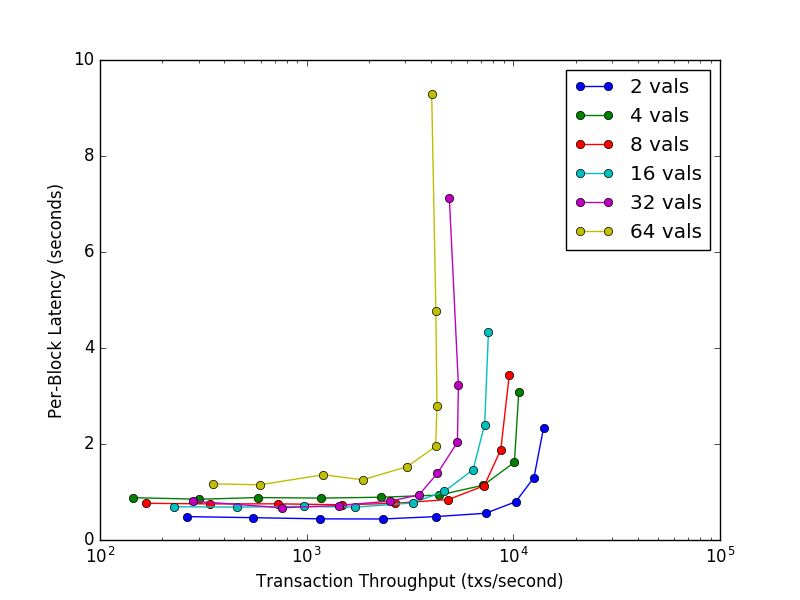
\includegraphics[width=\linewidth,height=\textheight,keepaspectratio]{figures/throughput/latency-throughput.png}
	\end{subfigure}

	\begin{subfigure}{0.8 \textwidth}
		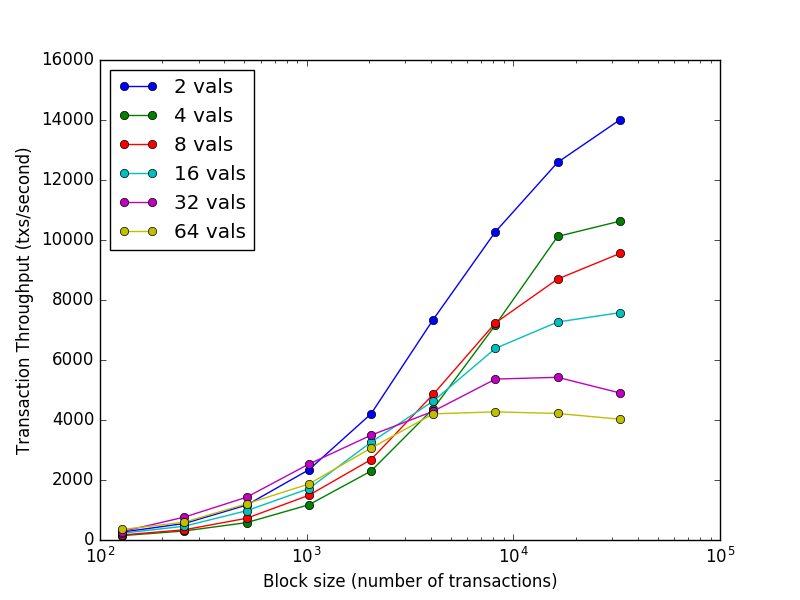
\includegraphics[width=\linewidth,height=\textheight,keepaspectratio]{figures/throughput/throughput-blocksize.png}
	\end{subfigure}
	\centering
	\caption[Latency-Throughput tradeoff in non-faulty global network]{Larger blocks incur diminishing 
returns in transaction throughput, with an ultimate capacity at around 10,000 txs/s}
	\label{fig:exp:throughput}
\end{figure}

As can be seen in Figure \ref{fig:exp:throughput},
Tendermint easily handles thousands of transactions per second with around one second block latency,
though there appears to be a capacity limit at around ten thousand transactions per second.
A block of 16384 transactions is about 4 MB in size, and analysis of network bandwidth shows each connection
easily reaching upwards of 20MB/s, though analysis of the logs shows that at high block sizes, 
validators can spend upwards of two seconds waiting for block parts.
Additionally, experiments in single data centers, as shown in Figure \ref{fig:exp:throughput:single},
demonstrate that much higher throughputs are possible,
while experiments on much larger machines, with 32 vCPU, exhibit more consistent performance,
relieving the capacity limit, as shown in Figure \ref{fig:exp:throughput:large}.
We leave further investigations of this capacity limit to future work.

\begin{figure}[]
	\centering
	\begin{subfigure}{0.8 \textwidth}
		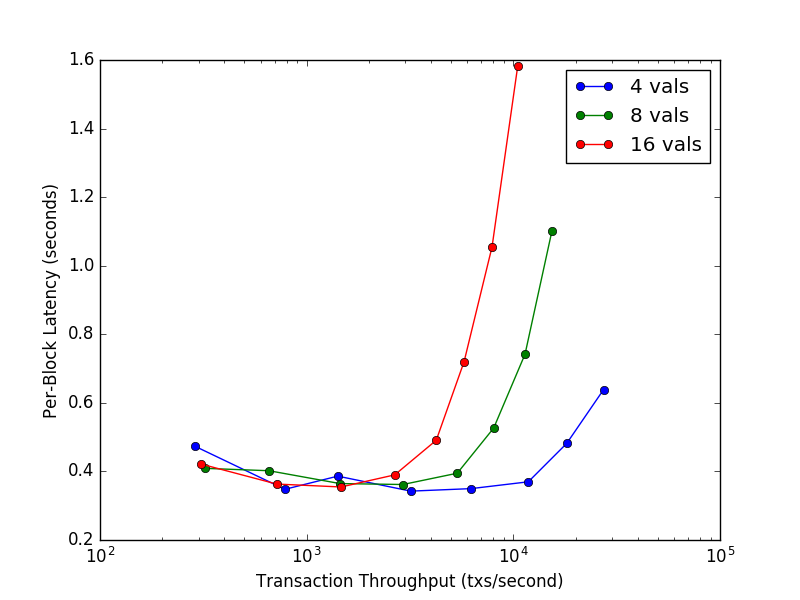
\includegraphics[width=\linewidth,height=\textheight,keepaspectratio]{figures/throughput/single_datacenter/latency-throughput.png}
		\centering
	\end{subfigure}

	\begin{subfigure}{0.8 \textwidth}
		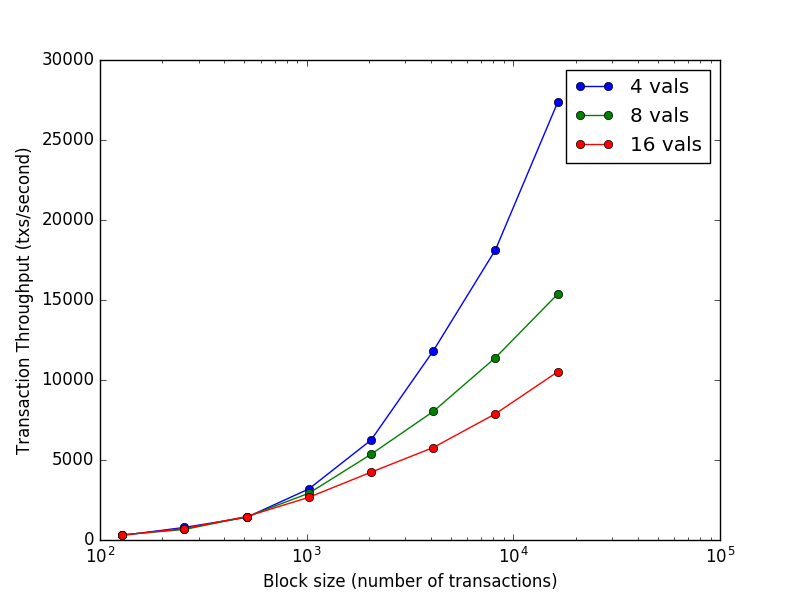
\includegraphics[width=\linewidth,height=\textheight,keepaspectratio]{figures/throughput/single_datacenter/throughput-blocksize.png}
	\end{subfigure}
	\caption[Latency-throughput tradeoff in non-faulty local network]{Latency-throughput tradeoff in a single datacenter shows Tendermint is capable of tens of thousands of transactions per second.}
	\label{fig:exp:throughput:single}
\end{figure}



\begin{figure}[]
	\centering
	\begin{subfigure}{0.8 \textwidth}
		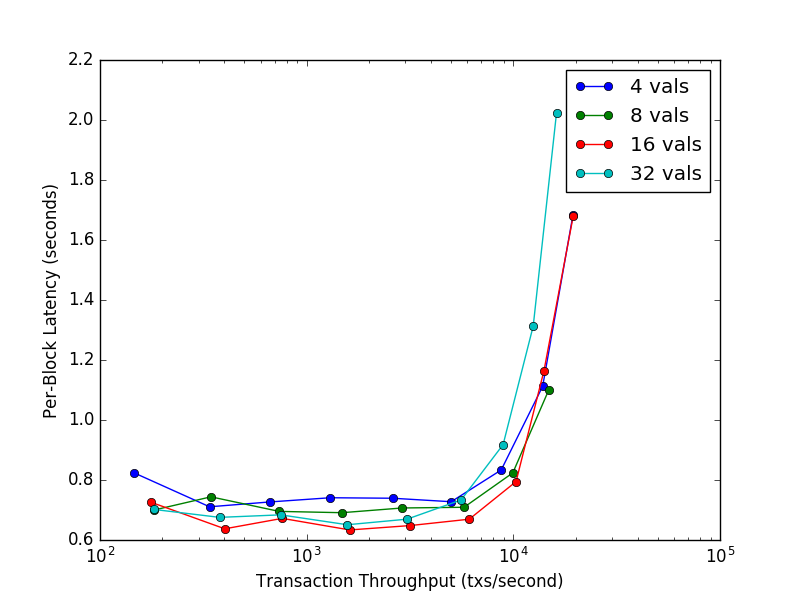
\includegraphics[width=\linewidth,height=\textheight,keepaspectratio]{figures/throughput/large_instances/latency-throughput.png}
		\centering
	\end{subfigure}

	\begin{subfigure}{0.8 \textwidth}
		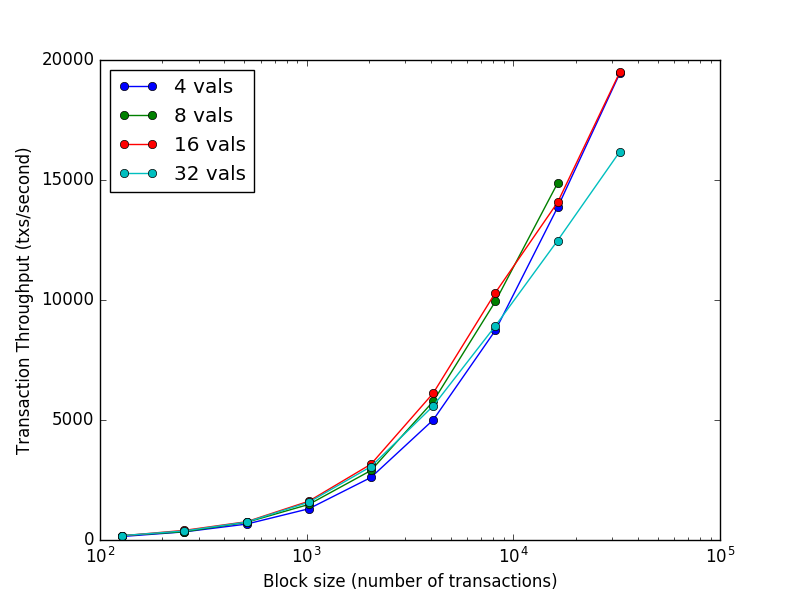
\includegraphics[width=\linewidth,height=\textheight,keepaspectratio]{figures/throughput/large_instances/throughput-blocksize.png}
	\end{subfigure}
	\centering
	\caption[Throughput-blocksize in non-faulty global network on large machines]{On larger machines, 
with 32 vCPU and 60 GB of RAM, transaction throughput increases linearly with block-size, 
relieving the capacity limits found on smaller machines.}
	\label{fig:exp:throughput:large}
\end{figure}

\section{Crash Failures}

To evaluate the performance of a network subject to crash failures, 
every three seconds $N_{fault}$ validators were randomly selected,
stopped, and restarted three seconds later.
Experiments are run for validator set sizes doubling from 2 to 32, for varying values of TimeoutPropose.
In each experiment, the block size is 2048.

The results in Table \ref{fig:exp:crash_failure} demonstrate that 
performance under this crash failure scenario drops by about 
$50\%$, and that larger TimeoutPropose values help mediate latencies. 
While the average latency increases to about two seconds,
the median is closer to one second, and latencies may run as high as ten or twenty seconds.


\ifx
Crash failures are closely related to asynchrony, as it can be difficult to distinguish between a crashed node
and delayed messages. A variety of heuristics exist, such as using pings, 
but in each case they require an assumption of some synchrony. 
To evaluate performance in the face of network asynchrony, twenty percent of all messages are delayed an amount of time chosen uniformly 
from one to ten seconds.
\fi

\begin{table}
	4 Validators

\begin{center}
	\begin{tabular}{| l | l | l | l | l | l | }
		\hline
		TimeoutPropose & Min & Max & Mean & Median & $95^{th} \ \%-ile$ \\ \hline
		500 & 434 & 15318 & 2179 & 1102 & 5575 \\ \hline
		1000 & 516 & 18149 & 2180 & 1046 & 5677 \\ \hline
		2000 & 473 & 15067 & 2044 & 1049 & 5479 \\ \hline
		3000 & 428 & 9964 & 2005 & 1096 & 5502 \\ \hline
	\end{tabular}
\end{center}

8 Validators

\begin{center}
	\begin{tabular}{| l | l | l | l | l | l | }
		\hline
		TimeoutPropose & Min & Max & Mean & Median & $95^{th} \ \%-ile$ \\ \hline
		500 & 618 & 126481 & 2679 & 990 & 5589 \\ \hline
		1000 & 570 & 9832 & 1763 & 962 & 5835 \\ \hline
		2000 & 594 & 8869 & 1658 & 968 & 5481 \\ \hline
		3000 & 535 & 10101 & 1633 & 959 & 5485 \\ \hline
	\end{tabular}
\end{center}

16 Validators

\begin{center}
	\begin{tabular}{| l | l | l | l | l | l | }
		\hline
		TimeoutPropose & Min & Max & Mean & Median & $95^{th} \ \%-ile$ \\ \hline
		500 & 782 & 21354 & 1977 & 1001 & 5930 \\ \hline
		1000 & 758 & 12659 & 1761 & 981 & 5642 \\ \hline
		2000 & 751 & 21285 & 2041 & 1005 & 6872 \\ \hline
		3000 & 719 & 72406 & 2395 & 991 & 5987 \\ \hline
	\end{tabular}
\end{center}

32 Validators

\begin{center}
	\begin{tabular}{| l | l | l | l | l | l | }
		\hline
		TimeoutPropose & Min & Max & Mean & Median & $95^{th} \ \%-ile$ \\ \hline
		500 & 760 & 24692 & 2591 & 1087 & 14025 \\ \hline
		1000 & 755 & 19696 & 2328 & 1119 & 9321 \\ \hline
		2000 & 852 & 21044 & 2178 & 1141 & 6514 \\ \hline
		3000 & 763 & 25587 & 2289 & 1119 & 6707 \\ \hline
	\end{tabular}
\end{center}


	\caption[Latency statistics under crash faults]{Crash-fault latency statistics. Every three seconds, a random selection of$N_{fault}$ validators were crashed, and restarted three seconds later. This crash-restart procedure continued for 200 blocks. Each table reports the minimum, maximum, average, median, and $95^{th}$ percentile of the block latencies, for varying values of the TimeoutPropose parameter.}
	\label{fig:exp:crash_failure}
\end{table}


\section{Byzantine Failures}

Since it is infeasible to capture every instance of arbitrary behaviour,
a single implementation is provided which covers some important cases.
The consensus state machine is augmented to allow explicit Byzantine behaviour,
by making the following changes:

\begin{itemize}
\item{Conflicting proposals: during its time to propose, a Byzantine validator signs two conflicting proposals and broadcasts each, along with a prevote and precommit, to separate halves of its connected peers.} 
\item{No nil votes: a Byzantine validator never signs a nil-vote.}
\item{Sign every proposal: a Byzantine validator submits a prevote and a precommit for every proposal it sees, as soon as it sees it.}
\end{itemize}

Taken together, these behaviours explicitly violate the double signing and locking rules. 
Despite these faults, which would cause many systems to fail completely and immediately,
Tendermint maintains respectable latencies, in some cases better and in others worse than crash faults (Table \ref{fig:exp:byz_failure})

\begin{table}[]
	
\begin{subtable}{.5 \linewidth}
	\centering
	\begin{tabular}{| l | l | l | l | l | l | }
		\hline
		TimeoutPropose & Min & Max & Mean & Median & $95^{th} \ \%-ile$ \\ \hline
		1000 & 868 & 3888 & 1450 & 1086 & 3320 \\ \hline
		2000 & 929 & 4375 & 1786 & 1272 & 4166 \\ \hline
		3000 & 881 & 4363 & 1224 & 1099 & 1680 \\ \hline
		4000 & 824 & 8256 & 1693 & 1272 & 2607 \\ \hline
	\end{tabular}
	\caption{4 Validators}
\end{subtable}


\begin{subtable}{.5 \linewidth}
	\centering
	\begin{tabular}{| l | l | l | l | l | l | }
		\hline
		TimeoutPropose & Min & Max & Mean & Median & $95^{th} \ \%-ile$ \\ \hline
		1000 & 771 & 3445 & 1472 & 916 & 3288 \\ \hline
		2000 & 731 & 3661 & 1426 & 902 & 3339 \\ \hline
		3000 & 835 & 6402 & 1912 & 962 & 6155 \\ \hline
		4000 & 811 & 4462 & 1512 & 964 & 3592 \\ \hline
	\end{tabular}
	\caption{8 Validators}
\end{subtable}


\begin{subtable}{.5 \linewidth}
	\centering
	\begin{tabular}{| l | l | l | l | l | l | }
		\hline
		TimeoutPropose & Min & Max & Mean & Median & $95^{th} \ \%-ile$ \\ \hline
		1000 & 877 & 15930 & 2086 & 1024 & 5844 \\ \hline
		2000 & 808 & 5737 & 1580 & 1027 & 4155 \\ \hline
		3000 & 919 & 10533 & 1801 & 1110 & 4174 \\ \hline
		4000 & 915 & 5589 & 1745 & 1095 & 4181 \\ \hline
	\end{tabular}
	\caption{16 Validators}
\end{subtable}


\begin{subtable}{.5 \linewidth}
	\centering
	\begin{tabular}{| l | l | l | l | l | l | }
		\hline
		TimeoutPropose & Min & Max & Mean & Median & $95^{th} \ \%-ile$ \\ \hline
		1000 & 1594 & 11730 & 2680 & 1854 & 5016 \\ \hline
		2000 & 1496 & 17801 & 3430 & 1874 & 11730 \\ \hline
		3000 & 1504 & 15963 & 3280 & 1736 & 9569 \\ \hline
		4000 & 1490 & 24836 & 3940 & 1773 & 12866 \\ \hline
	\end{tabular}
	\caption{32 Validators}
\end{subtable}


	\caption[Latency statistics under byzantine faults]{Byzantine-fault latency statistics.
Byzantine validators propose conflicting blocks and vote on any proposal as soon as they see it.
Each table reports the minimum, maximum, average, median, and $95^{th}$ percentile of the block latencies, for varying values of the TimeoutPropose parameter.}
	\label{fig:exp:byz_failure}
\end{table}

\section{Random Network Delay}

Another form of fault, which may attributed either to Byzantine behaviour or to network asynchrony,
is to inject random delays into every read and write to a network connection.
In this experiment, before every read and write on every network connection,
a faulty validator slept for $X$ milliseconds, where $X$ is drawn uniformly on $(0, 3000)$.
As can be seen in Table \ref{fig:exp:delay}, 
performance drops to a thousand transaction per second, falling further with largest TimeoutPropose values.
The drop in 

\begin{table}[]
	
\begin{subtable}{.5 \linewidth}
	\centering
	\begin{tabular}{| l | l | l | l | l | l | }
		\hline
		TimeoutPropose & Min & Max & Mean & Median & $95^{th} \ \%-ile$ \\ \hline
		1000 & 873 & 2796 & 1437 & 1036 & 2627 \\ \hline
		2000 & 831 & 4549 & 1843 & 1180 & 4036 \\ \hline
		3000 & 921 & 5782 & 2273 & 1251 & 5491 \\ \hline
		4000 & 967 & 6875 & 2700 & 1413 & 6781 \\ \hline
	\end{tabular}
	\caption{4 Validators}
\end{subtable}


\begin{subtable}{.5 \linewidth}
	\centering
	\begin{tabular}{| l | l | l | l | l | l | }
		\hline
		TimeoutPropose & Min & Max & Mean & Median & $95^{th} \ \%-ile$ \\ \hline
		1000 & 870 & 2840 & 1449 & 1040 & 2786 \\ \hline
		2000 & 957 & 4268 & 1848 & 1076 & 4148 \\ \hline
		3000 & 859 & 5724 & 2156 & 1100 & 5649 \\ \hline
		4000 & 897 & 11859 & 3055 & 1093 & 11805 \\ \hline
	\end{tabular}
	\caption{8 Validators}
\end{subtable}


\begin{subtable}{.5 \linewidth}
	\centering
	\begin{tabular}{| l | l | l | l | l | l | }
		\hline
		TimeoutPropose & Min & Max & Mean & Median & $95^{th} \ \%-ile$ \\ \hline
		1000 & 914 & 5595 & 1821 & 1135 & 5466 \\ \hline
		2000 & 950 & 7782 & 2490 & 1165 & 7650 \\ \hline
		3000 & 978 & 10305 & 3049 & 1163 & 9890 \\ \hline
		4000 & 1018 & 6890 & 2808 & 1174 & 6813 \\ \hline
	\end{tabular}
	\caption{16 Validators}
\end{subtable}


\begin{subtable}{.5 \linewidth}
	\centering
	\begin{tabular}{| l | l | l | l | l | l | }
		\hline
		TimeoutPropose & Min & Max & Mean & Median & $95^{th} \ \%-ile$ \\ \hline
		1000 & 1202 & 8562 & 2219 & 1349 & 5733 \\ \hline
		2000 & 1196 & 7878 & 2549 & 1365 & 7579 \\ \hline
		3000 & 1164 & 10082 & 3003 & 1382 & 9805 \\ \hline
		4000 & 1223 & 17571 & 3696 & 1392 & 12014 \\ \hline
	\end{tabular}
	\caption{32 Validators}
\end{subtable}


	\caption[Latency statistics under randomized delays]{Random delay latency statistics. $N_{fault}$ validators were set to inject a random delay
before every read and write, where the delay time was chosen uniformly on $(0, 3000)$ milliseconds.}
	\label{fig:exp:delay}
\end{table}

\ifx
\section{A real application: ErisDB}

The experiments presented so far have been artificial to the extent that transactions incur no processing logic.
This was done deliberately to benchmark the core consensus engine. 
To get a handle on a real application, we present throughput and latency results for ErisDB, 
a blockchain application developed primarily by the author at Eris Industries, in collaboration with Jae Kwon.
ErisDB provides a rich set of features, including a native currency, the Ethereum Virtual Machine (EVM).
a native name registry, and a rich permissioning system.
Transactions must be digitally signed using ED25519 signatures to be valid, and all state queries and updates are done on a merkle IAVL tree.

For this experiment, a simple contract with two methods, get and set, is deployed to the virtual machine.
The contract is written in solidity, a high-level, javascript-like language developed by Ethereum which compiles down to EVM byte code.
The application state is preloaded with 1000 accounts, and transactions are signed by private keys drawn uniformly from those accounts.
Keys and values for the get and set methods are fixed at 32-bytes each, to reflect the native architecture of the EVM \cite{ethereum_yellow_paper}.
Transactions are generated for a read/write load of 10/90 (i.e. 90\% of transaction call the set method).

\fi

\section{Related Work}

The experiments in this chapter were modeled after those in \cite{honeybadger},
which benchmarks the performance of a PBFT implementation and a new randomized BFT protocol called HoneyBadgerBFT.
In their results, PBFT achieves over 15,000 transactions per second on four nodes,
but decays exponentially as the number of nodes increases, while HoneyBadgerBFT attains roughly even performance
of between 10,000 and 15,000 transactions per second.
Block latencies in HoneyBadgerBFT, however, are much higher, 
closer to 10 seconds for validator sets of size 8, 16, and 32, and even more for larger ones.

The author is not aware of any throughput experiments in the face of persistent crash or Byzantine failures,
like those presented here.

\section{Conclusion}

The implementation of Tendermint written by the author and Jae Kwon easily achieves 
thousands of transactions per second on up to 64 nodes on machines distributed around the globe, 
with latencies mostly in the one to two second range.
This is highly competitive with other solutions, and especially with the current state of blockchains,
with Bitcoin, for instance, capping out at around 7 transactions per second.
Furthermore, our implementation is shown to be robust to both crash faults and deliberate Byzantine faults,
being able to maintain over a thousand transactions per second in the face of either scenario.



\chapter{Related Work}
\label{ch:related}

Byzantine consensus has a rich history that spans cryptography, distributed computing, and economics,
but the socio-economic context for its products to be deployed in industry has not existed until recently,
at least not outside of traditionally critical real-time systems like air-craft control \cite{draper_lab}.
On the one hand, the invention of Bitcoin and the coining of the term ``blockchain'' popularized the notion
of a distributed ledger not controlled by a single entity, using cryptography and aligned economic incentives to 
preserve safety in the face of Byzantine faults.
On the other, the continued commoditization of servers, in the form of ``The Cloud'', and the invention of Raft, 
have popularized distributed computing in mainstream developer culture, 
and brought renewed attention to distributed consensus algorithms as co-ordination hubs in large-scale deployments. 

At the intersection are a collection of solutions, typically geared for banking and financial applications,
but also for governance, logistics, and other general forms of co-ordination, 
that draw on classic academic BFT modified and modernized in various ways.
This chapter reviews the history and diversity of these ideas, with the goal of providing a rich context within which to 
understand the blockchain phenomenon.

\section{Beginnings}

Distributed algorithms first emerged in the late 19th century in the telecommunications and railroad industries,
in attempts to effectively handle multiple concurrent message streams in a transmission, 
or multiple trains on the same set of tracks.

Academic work on the subject appears to have been launched officially by the seminal work
of Edsger Dijkstra on the mutual exclusion problem \cite{mutex}, and of Tony Hoare on models for describing communicating processes.\cite{csp}, 

A host of concurrency problems with catchy names were popularized around this time,
including the cigarette smokers problem \cite{cigarette_smokers}, where smokers sit around a table, 
each with a different ingredient, and must successfully roll a full cigarette,
the dinning philosophers problem \cite{dining_philosophers},
where philosophers sitting around a table must take turns eating and thinking,
but each can only eat while its neighbours are thinking,
and the two-generals or co-ordinated attack problem \cite{gettier},
where two generals must co-ordinate from afar to attack an enemy city at the same time.

These problems served to put the focus on synchronization primitives
such as semaphores, mutexes, and communication channels,
and would lay the ground for a number of advancements over the coming decades.

\subsection{Faulty Things}

Fault tolerant distributed computing effectively emerged in the late seventies 
out of the effort to utilize microprocessors for aircraft control, resulting in a number of early systems \cite{sift,ftmp}.
Today, it is standard for NASA to conduct BFT research \cite{miner2004unified}, 
and for commercial aircraft to use BFT systems, such as the SAFEbus \cite{hoyme1993safebus}.

Many systems, however, do not require tolerance to Byzantine faults as they are run in controlled environments,
where there is presumably no malicious behaviour and the code is written correctly.
In these circumstances, which are common in data-centers managed by large companies like Google or Amazon,
fault tolerant computing is used to defend against various faults,
whether it be a break in a network link, power failure in a server rack, or a dead harddrive.

\subsection{Clocks}

The problem of distributed consensus, however, did not formally emerge until Leslie Lamport introduced it in his 
``Time, clocks, and the ordering of events in a distributed system'' \cite{clocks}.
In that work, Lamport demonstrated how a partial ordering of events emerges from a definition of causality based on communication \cite{clocks}.
That is, events occurring in concurrent processes, between communication events, 
effectively happen at the same time, as they cannot influence one another.
Thus, a system of logical clocks can be defined based on the individual sequential processes 
and the fact that messages are sent before they are received.
Events can then be totally ordered by assigning any arbitrary but consistent total ordering above the partial ordering,
for instance by assigning each process in the system an index and ordering events which happen at the same logical time by the
index of the process in which they happen.
The algorithm is quite simple, requiring each process to hear from each other process in order to determine the order of events.

Lamport's work established time as a principle obstacle to designing fault tolerant distributed systems,
as synchronizing clocks across geographical locations requires the communication of messages 
which is ultimately limited by the speed of light.
This formulation of the problem has close ties to the relativism of modern physics,
wherein frames of reference are relative to an observer and the speed of light imposes a constraint on information propagation.

\subsection{FLP}
As discussed in Chapter \ref{ch:motivation}, 
one of the primary factors in designing consensus algorithms are assumptions made about 
network and/or processor synchrony. 
A synchronous network is one in which messages are delivered within some fixed, 
known amount of time. 
Similarly, synchronous processors are one whose clocks stay within some fixed, 
known number of ticks of eachother.
In the early days of consensus research, the distinction was not well characterized, 
though the close relationship between asynchrony and crash failures is apparent even in \cite{clocks}.
Lamport's original consensus algorithm is able to operate in asynchronous environments, 
so long as all messages are eventually delivered from each process.
However, the algorithm is obviously not fault tolerant as the failure of just a single process can halt the algorithm forever.

The intuition behind a single failure thwarting a consensus protocol was given formal ground by Fischer, Lynch, and Patterson,
who proved the impossibility of deterministic distributed consensus in asynchronous environments if even a single process can fail \cite{flp}.
The result does not apply to synchronous contexts, 
as assumptions about network synchrony allow processors to detect failures using timeouts, 
such that if a process does not respond within some given amount of time it is assumed to have crashed.
Furthermore, the result applies to deterministic consensus protocols only, 
as its proof relies on the moment when the network goes deterministically from a bivalent state, 
where not all processes hold the same value, to a univalent one, where they do.
Since the point of transition is a deterministic point in time, 
consensus fails if a single processes crashes at that opportune moment.

\subsection{Common Coin}

The FLP result became something of a warning bell to distributed systems scientists, 
establishing a clear impossibility result at the heart of the emerging field.
Later, the approach would be generalized to derive many more impossibility results \cite{impossibility},
and significant academic effort would be expended on relaxing either the synchrony or determinism assumptions to derive algorithms which circumvent the result.

In particular, in a short note, 
Ben Or demonstrated how an algorithm which includes a simple amount of non-determinism can circumvent the FLP result \cite{free-choice}.
The algorithm is tolerant to faults of up to half of the processes in asynchronous environments.
Essentially, in trying to reach consensus on the value of a single bit, 
if a process does not receive votes from a majority for the same value, it randomly changes the value it votes for the next round.
With everyone changing values, eventually more than half of them will vote the same value.
This approach came to be known as a \emph{common coin},
due to the resemblance of the procedure to communally flipping a coin to obtain a shared value.

The problem with Ben Or's common coin is that, in the asynchronous case,
the algorithm requires a number of rounds exponential in the number of validators.
This was quickly rectified in a follow up by Rabin, who showed how a common coin
could be constructed using secret sharing, as pioneered by Shamir \cite{shamir1979share},
to achieve consensus in a fixed number of rounds \cite{rabin1983randomized}.
The approach is useful for BFT as well, and is discussed more fully in that context in a later section.

\subsection{Transaction Processing}

Parallel to the development of fault tolerant consensus algorithms was the emergence of the first commercial database systems.
While they did not at first use the consensus protocols being developed, 
they built atop the growing body of work in distributed computing and concurrency.
In particular is the seminal work of Jim Gray, who introduced the term \emph{transaction} 
as an atomic unit of work in a database system \cite{gray1981transaction}. 
That is, a transaction is either applied in full or not at all.

Jim also introduced other classic features of modern databases,
such as the principles of Atomicity, Consistency, Isolation, and Durability, 
which come part and parcel with the transaction concept \cite{gray1981transaction},
and the use of write-ahead-logs, for logging transactions to disk before they are executed
in order to recover from faults occurring during transaction execution \cite{gray1978notes}.

In a distributed database setting, this work on transactions, atomicity, and consistency
led to a series of approaches for database replication centered around the notion of an \emph{atomic commit},
wherein a transaction is replicated atomically across all machines.
These approaches are known as two-phase-commit \cite{gray1978notes}, and its non-blocking alternative,
three-phase-commit \cite{skeen1983formal}.

Both two-phase and three-phase commit protocols work only in a synchronous setting,
where crash failures can be detected, and utilize a co-ordinator process that serves as leader for the protocol.

\subsection{Broadcast Protocols}

The problem of ordering a set of transactions in a distributed setting subject to faults has also been known as 
the problem of \emph{total order broadcast} or \emph{atomic broadcast} \cite{defago2004total}.
In particular, an atomic broadcast protocol is expected to satisfy the following properties:

\begin{itemize}
\item{Validity}: if a correct process broadcasts a message, it is eventually received.
\item{Agreement}: if a process receives a message, then all correct processes eventually receive that message.
\item{Integrity}: a message is received at most once by a process, and only if it was sent by another process.
\item{Total Order}: if two messages are received by two processes, the messages are received in the same order.
\end{itemize}

Atomic broadcast is built above a simpler primitive, known as \emph{reliable broadcast}, 
the difference being that atomic broadcast ensures the messages are totally ordered,
while reliable broadcast ensures only that the messages are delivered.
That is, reliable broadcast satisfies all the above properties except the final one.
A taxonomy and survey of solutions to the problem is provided in \cite{defago2004total}.

\section{Byzantine}
Many fault tolerant protocols focus only on crash failures, as they are the most common,
while much less attention has been given to the problem of potentially arbitrary, including malicious,
behaviour of software. This more general problem is known as Byzantine Fault Tolerance.

\subsection{Byzantine Generals}

Lamport introduced the problem of Byzantine Fault Tolerance in \cite{pease1980reaching},
but gave the problem its name in a later paper by making an analogy with the problem faced
by the Byzantine army in co-ordinating to attack an enemy city \cite{lamport1982byzantine}.
The army is composed of multiple divisions, each of which is led by a general.
Communication between generals happens only via messenger.
How can the generals agree on a common plan of action if one or some of the generals is a traitor?

The original paper provides the first proof that to tolerate $f$ Byzantine faults,
a system must have at least $3f+1$ nodes. 
The intuition behind this result was depicted in \ref{fig:byzantine} and discussed 
throughout Chapters \ref{ch:motivation} and \ref{ch:tendermint}.
A number of algorithms are provided in both papers as the first solutions to the problem,
though they are designed to work only in the synchronous case, where the absence of a message can be detected.

\subsection{Randomized Consensus}

Asynchronous Byzantine consensus saw its first solution in the form of the common coins
introduced by Ben Or \cite{free-choice} and Rabin \cite{rabin1983randomized}.
However, neither solution achieves optimal Byzantine fault tolerance of $3f+1$ machines for $f$ faults.
Ben Or's solution requires $5f+1$ machines, while Rabin's requires $10t+1$ machines.
The solution was iteratively improved to achieve optimal Byzantine agreement with low overhead \cite{feldman1988optimal,canetti1993fast,cachin2000random}.

\subsection{Partial Synchrony}

The next major advancement in BFT came in the form of the so called \emph{DLS} consensus algorithms,
named after the authors Dwork, Lynch, and Stockmeyer \cite{DLS}.
The innovation of DLS was to define a middle ground between synchrony and asynchrony called \emph{partial synchrony}.
Recall from Chapter \ref{ch:motivation} that a synchrony assumption is one which states that messages 
are received within some known, finite amount of time, 
or that processor clocks only deviate from eachother by some finite number of ticks.
The secret to partial synchrony is to suppose one of the following:

\begin{itemize}
\item{Messages are guaranteed to be delivered within some fixed but unknown amount of time.}
\item{Messages are guaranteed to be delivered within some known amount of time, beginning an unknown amount of time in the future.}
\end{itemize}

The DLS algorithm proceeds via series of rounds, each of which is divided into \emph{trying} and \emph{lock-release} phases.
Each round has a corresponding proposer, and processes can \emph{lock} on a value at a round if they think
the proposer will propose that value.
A round begins with processes gossiping the values they deem acceptable.
The proposer will propose a value if it has heard from at least $N - f$ processes that the value is acceptable.
Any process which receives the proposed value should lock on it, and send an acknowledgement message
that it has done so.
If the proposer receives acknowledgement from $f+1$ processes, it commits the value.

Variations on the basic protocol are discussed for different combinations of assumptions,
and many proofs are provided of its soundness.
Despite its success, however, DLS algorithms were never widely adopted for BFT.
Tendermint's original design was based on DLS, in particular the version which assumes
a partially synchronous network but synchronous processor clocks.
In practice, due to the use of protocols like the Network Time Protocol (NTP), 
synchronized clocks may be a fair assumption.
However, NTP is vulnerable to a number of attacks,
and protocols which assume synchronous clocks can be slow to recover from crash faults.
In the summer of 2015, the core Tendermint consensus protocol was redesigned to be more fully asynchronous,
as described in \ref{ch:tendermint},
and has thus come to more closely resemble another BFT algorithm,
known as Practical Byzantine Fault Tolerance (PBFT).

\subsection{PBFT}

PBFT was introduced in 1999 \cite{pbft}, and was widely hailed as the first practical BFT algorithm,
suitable for use in asynchronous networks,
though it does in fact make weak synchrony assumptions which can be violated by a careful adversary \cite{honeybadger}.
PBFT proceeds through a series of views, 
where each view has a proposer, known as a primary,
that is selected in round-robin order.
The primary receives requests from clients,
assigns them a sequence number, and broadcasts a signed \emph{pre-prepare}
messages to the other processes containing the view and sequence numbers.
Replicas accept the \emph{pre-prepare} message if they have not already accepted one for the same
view and sequence numbers, assuming the message is for the current view and signed by the correct primary.

Once a \emph{pre-prepare} is accepted, a replica broadcasts a signed \emph{prepare} message.
A replica is said to be \emph{prepared} for a given client request when it has received $2f$ \emph{prepare}
messages for that request, with the same view and sequence number.
The combination of \emph{pre-prepare} and \emph{prepare} ensure a total order on the requests in a single view,
according to their sequence number. 
Once a replica is prepared, it broadcasts a signed \emph{commit} message,
which is accepted so long as its properly signed and the view is correct.
When a replica accepts a \emph{commit} message, it runs the client request against the state machine and returns the result to the client.

PBFT employs an additional mechanism to facilitate view changes in the event the primary is faulty.
Replicas maintain a timeout, which restarts every time they receive a new client request, 
and terminates when a \emph{pre-prepare} is received for that request.
If no \emph{pre-prepare} is received, the replica  times out, and triggers the view change protocol.
View change is subtle and somewhat complicated as it requires consensus that the view should be changed, 
and all client requests since the last commit must be brought into the new view.

Tendermint side-steps these issues through the use of blocks and by changing proposers every block,
allowing a proposer to be skipped using the same mechanism used to commit the proposed block.
Furthermore, the use of blocks allows Tendermint to include the set of \emph{pre-commit} 
messages from one block in the next block, removing the need for an explicit \emph{commit} message.

\subsection{BFT Improvements} 

Many improvements have been proposed for PBFT since it was published.
Some of these focus on so-called \emph{optimistic execution}, 
where transactions are executed before they are committed in order to provide a low-latency,
optimistic reply to clients \cite{kotla2007zyzzyva,garcia2011efficient}.
The trouble with these approaches is that the responsibility of managing inconsistency is relegated to the client,
while presumably the reason they used a consistent consensus protocol in the first place was to avoid that responsibility.
Alternatively, this may be a useful approach in low-fault circumstance.
The phenomenon is referred to as \emph{zero-conf transactions} in Bitcoin and is widely warned against,
given Bitcoin's weak consistency guarantees.

Others have focused on the possibility of running indepedent transactions concurrently to achieve higher throughputs \cite{kotla2004high}.
This is the approach that has begun to be researched in the blockchain community, especially by Ethereum, in order to produce a scalable blockchain architecture.

\section{Non-Byzantine}

In parallel to the BFT algorithms, a number of non-BFT algorithms have emerged, and a 
number of important highly available internet services have been built on top of them.

\subsection{Paxos}

It is often said in consensus science that there is only one consensus algorithm, and it is Paxos.
This is on the one hand a statement of the significance of the Paxos algorithm to the field,
and on the other a reflection on the universal foundation of consensus protocols,
which is in every case ``Paxos-like''.

Lamport introduced Paxos in the early nineties, though the article was not accepted for publication until 
almost a decade later \cite{paxos}.
Many have pointed out that the algorithm is actually quite similar to Viewstamped Replication,
published in the late eighties \cite{oki1988viewstamped},
and that the two represent independent discovery of the same protocol.

The protocols are quite similar to PBFT, which came after them, 
but require only $2f+1$ machines to tolerate $f$ faults as they are not BFT.
Another similar protocol, the Zookeeper Atomic Broadcast protocol (ZAB) \cite{junqueira2011zab}
was developed for the Apache Zookeeper distributed key-value store.
The similarities and differences of each algorithm are illuminated in \cite{van2015vive}.

\subsection{Raft} 

Non-BFT consensus science received a major improvement with the introduction of Raft \cite{raft},
which was designed from ground up to be \emph{understandable}, 
and which even proved itself to be more understandable than Paxos through a user survey \cite{raft_thesis}.

Raft is similar in spirit to Paxos and Viewstamped Replication, but it emphasizes replicating a transaction log, 
rather than a single bit, and introduces randomization for more efficient leader elections.
Furthermore, Raft's safety guarantees have been formally proven using the Coq proof assistant \cite{woos2016planning}
and a framework built above Coq, called Verdi, for formally verifying distributed systems \cite{wilcox2015verdi}.

\section{Blockchain}

This thesis was motivated by the introduction of blockchain technology, which emerged in the form of Bitcoin,
and has since seen many iterations.
Few have succeeded in putting the blockchain in context of classical consensus science until recently \cite{vukolic11quest,cachin2016non,honeybadger}.

\subsection{Bitcoin} 

Bitcoin was the first blockchain, introduced in \cite{bitcoin}.
It solved the atomic broadcast problem in a public, adversarial setting through a clever use of economics.
In particular, the order of transactions comes in blocks proposed by those who solve partial hash collisions,
where the data being hashed is the block of transactions.
Since computing partial hash collisions is expensive, requiring brute force search in a large space,
the effort is subsidized by the issuance of a currency, known as bitcoins, with every block.
The protocol has been wildly successful, with the currency achieving a market capitalization
of roughly five billion dollars (USD), and with many clones of the original that have market capitalizations in the millions.

However, Bitcoin is not without it's issues. A number of design flaws make the protocol cumbersome and difficult 
for application developers to work with.
Furthermore, a number of academic works have shed light on incentive incompatibilities in the protocol,
weakening widely held assumptions about the protocol's security \cite{eyal2014majority,courtois2014subversive}.

Numerous approaches have been proposed to improve Bitcoin,
including those that change the nature of the partial hash collision function \cite{miller2015nonoutsourceable},
those that change the nature of leadership election in the protocol to improve many features of the economics and underlying performance \cite{eyal2015bitcoin}
and those that aim to augment the protocol in an effort to achieve scalability \cite{back2014enabling,poon2015bitcoin}.

\subsection{Ethereum}

Ethereum was introduced by Vitalik Buterin as a solution to the proliferation of cryptocurrencies that followed Bitcoin,
with different varieties of features \cite{buterin2013ethereum}.
Ethereum sought a more pure mandate: to have no features.
Instead, Ethereum provides a Turing complete virtual machine, the Ethereum Virtual Machine (EVM), for transaction execution above the consensus,
and provides a means for users to upload code to the EVM that can execute upon the processing of future transactions.
So-called \emph{smart contracts} \cite{} offer the promise of automatically enforced execution of code in a public setting, 
using strong cryptography and BFT replication. 
The Ethereum project was successful in one of the largest crowdfunds to date, over \$18 million USD, 
and the market capitalization of its native token, ether, which is used to pay for transaction execution and code uploads,
has since reached \$1 billion USD.

Ethereum currently uses a modified form of Proof-of-Work called Greedy Heaviest Observed Sub Tree (GHOST) \cite{ghost},
but is planning to move to a more secure economic consensus algorithm modeled around Proof of Stake.

\subsection{Proof-of-Stake}
...

\subsection{HyperLedger}

The success of Bitcoin, Ethereum, and other cryptocurrencies has inspired an increasingly diverse cross section of society,
including regulators, bankers, business executives, auditors, account managers, logisticians, and more.
In particular, a recent project under the Linux Foundation, spearheaded by IBM and a new blockchain-based company called Digital Asset Holdings (DAH), 
seeks to provide a unified blockchain architecture for industrial applications. The project is called HyperLedger,
after a company with the same name, thought provided a rudimentary implementation of a PBFT-based blockchain, was acquired by DAH.

Two contributions to the HyperLedger initiative are particularly relevant.
The first is the combination of Juno and Hopper by the team at JP Morgan.
Juno is an implementation of Tangaroa, a BFT version of Raft \cite{tangaroa},
Hopper is a new virtual machine design,
based on linear logic \cite{girard1987linear} and dependent type systems \cite{bove2009dependent},
that aims to provide an execution environment for smart contract systems equipped with a formal logic
for making and proving statements about the state of the system, or the behaviour of a contract.
Both Juno and Hopper are written in Haskell.

The other project is the OpenBlockchain by IBM, a PBFT-based blockchain written in Go,
sporting an application state that supports the deployment of arbitrary docker containers.
Since an arbitrary docker container may container non-determinism, their PBFT implementation
was modified with additional steps to preserve safety in the face of possibly non-deterministic execution \cite{cachin2016non}

Another relevant contribution from IBM is a recent review paper, similar in spirit to this chapter \cite{vukolic11quest}.

\subsection{HoneyBadgerBFT}

All Paxos like consensus protocols, including Raft, PBFT, and Tendermint, 
despite functioning well in asynchronous environments, are not strictly asynchronous.
This is because each one uses a timeout somewhere in the protocol, typically to detect faulty leaders.
On the other hand, randomized consensus protocols like the common coin offer solutions that work in 
a fully asynchronous context, with no timeouts.

All consensus protocols rely one way or another on the eventual delivery of messages.
The assumption of asynchrony simply states that there is no upper bound on when a message will be delivered.
Most of the time, networks act synchronous, in the sense that most messages are delivered within some bound.
The difference between a fully asynchronous protocol and one with timeouts is that 
an asynchronous protocol can \emph{always make progress} during times when the network is behaving synchronously.
This point is illustrated clearly in \cite{honeybadger}, which introduces HoneyBadgerBFT, 
the first fully asynchronous blockchain design, based on common coin consensus.

An adversary with arbitrary control over the network, 
and the ability to crash any one node at a time,
can cause PBFT to halt for arbitrarily long.
This can be done by crashing the current primary/proposer/leader during times when the network is synchronous,
and bringing it back for periods of asynchrony.
The network still eventually delivers messages, with some average synchrony,
but with precise timing can stop all system progress.
The experiment is carried out on PBFT directly in \cite{honeybadger}, and would work similarly against Tendermint.

The solution to this problem is HoneyBadgerBFT, a fully asynchronous atomic broadcast protocol \cite{honeybadger}.
HoneyBadgerBFT utilizes a series of cryptographic techniques, including secret sharing, erasure coding, 
and threshold signatures to design a high performance asynchronous BFT consensus protocol.
However, it requires a trusted dealer for initial setup and for validator changes, 
and it relies on relatively new cryptographic assumptions about the hardness of certain problems that have 
yet to withstand the test of time.

\section{Conclusion}

Tendermint emerges from and complements a rich history of consensus science which spans the gamut of synchrony and fault-tolerance assumptions. 
The invention of the blockchain and of Raft have rekindled the fire in consensus research and spawned a new generation 
of protocols and software for co-ordination over the internet.

\chapter{Conclusion}

Byzantine Fault Tolerant consensus provides a rich basis upon which to build services 
that do not depend on centralized, trusted parties, and which may be adopted by society
to manage critical components of socioeconomic infrastructure.
Tendermint, as presented in this thesis, was designed to meet the needs of such systems,
and to do so in a way that is understandably secure and easily high performance,
and which allows arbitrary systems to have transactions ordered by the consensus protocol,
with minimal fuss.

Careful considerations are necessary when deploying a distributed consensus system,
especially one without an agreed upon central authority to mediate potential disputes and reset the system in the event of a crisis.
Tendermint seeks to address such problems using explicit governance modules and accountability guarantees,
enabling integration of Tendermint deployments into modern legal and economic infrastructure.

There is still considerable work to do. This includes formal verification of the algorithm's guarantees, 
performance optimizations, and architectural changes to enable the system to increase capacity with the addition of machines.
And of course, many, many TMSP applications remain to be built.

We hope that this thesis better illuminates some of the problems in distributed consensus and blockchain architecture,
and inspires others to build something better.



\appendix
\chapter{Appendix Title}


\appendix
\chapter{Appendix Title}



\bibliographystyle{IEEEtran}
\bibliography{consensus}

\end{document}
